% !TEX program = pdflatex
\documentclass[12pt,a4paper]{article}

% ── Packages ──────────────────────────────────────────────────────────
\usepackage[utf8]{inputenc}
\usepackage[T1]{fontenc}
\usepackage{lmodern}
\usepackage[margin=2.5cm]{geometry}
\usepackage{amsmath,amssymb}
\usepackage{graphicx}
\usepackage[font={small,it},labelsep=period]{caption}
\usepackage{subcaption}
\usepackage{booktabs}
\usepackage{tabularx}
\usepackage{float}
\usepackage{setspace}
\usepackage{parskip}
\usepackage[hidelinks]{hyperref}
\usepackage{natbib}
\usepackage{xcolor}
\usepackage{enumitem}
\usepackage{fancyhdr}
\usepackage{lastpage}
\usepackage{titlesec}
\usepackage{microtype}

\onehalfspacing

% ── Header / footer ──────────────────────────────────────────────────
\pagestyle{fancy}
\fancyhf{}
\fancyhead[L]{\footnotesize\textit{Hedonic Bias in Conceptualisation of Patient Well-Being}}
\fancyhead[R]{\footnotesize\thepage/\pageref{LastPage}}
\renewcommand{\headrulewidth}{0.4pt}

% ── Figure path ──────────────────────────────────────────────────────
\graphicspath{{../figures/}}

% ── Custom commands ──────────────────────────────────────────────────
\newcommand{\Ddelta}{$\Delta$}
\newcommand{\floatnote}[1]{\par\vspace{4pt}\begin{minipage}{\linewidth}\small\textnormal{Note. #1}\end{minipage}}

% ══════════════════════════════════════════════════════════════════════
\begin{document}

% ── Title block ──────────────────────────────────────────────────────
\begin{center}
{\LARGE\bfseries Hedonic Bias in the Conceptualisation of Patient Well-Being:}\\[6pt]
{\Large\bfseries Evidence for Convergence Toward Hedonic Optimisation\\[2pt]
in Western Mental Healthcare}\\[18pt]

{\large Stijn Van Severen\textsuperscript{1,*} \quad Thomas De Schryver\textsuperscript{1}}\\[8pt]
{\small\textsuperscript{1} Independent Researchers}\\[4pt]
{\small\textsuperscript{*} Corresponding author}\\[18pt]

\today
\end{center}

\vspace{10pt}

% ══════════════════════════════════════════════════════════════════════
\begin{abstract}
Clinical psychology relies on standardised psychometric scales to assess well-being, distress, and functioning, yet philosophical and empirical work increasingly distinguishes two irreducible traditions: the \textit{hedonic} tradition, equating well-being with pleasure, positive affect, and satisfaction, and the \textit{eudaimonic} tradition, foregrounding meaning, purpose, virtue, and personal growth. Using OpenAI's text-embedding-3-large model, we embedded 205 widely used clinical scales alongside six theoretically derived hedonic--eudaimonic dimension pairs and computed cosine-similarity differentials~($\Delta$) to quantify the degree to which Western clinical assessment over-represents hedonic constructs. Across all scales and dimensions, we found a large and consistent hedonic bias (mean $\Delta = +0.060$, Cohen's $d = 1.05$, $p < .001$; Wilcoxon signed-rank, Holm-corrected), robust to usage-weighting ($\Delta_w = +0.056$, $d = 1.07$), corpus-size variation ($d = 1.31$--$1.53$), and permutation testing ($p = .017$). Temporal analysis of PubMed publication counts (2000--2025) revealed that this bias has \textit{increased} over the past quarter-century (aggregate slope $= +5.5 \times 10^{-4}$/year, $R^2 = .96$, $p < .001$; Mann-Kendall $S = 321$, $p < .001$), with all six dimensions showing significant positive trends and domain-level analyses indicating that Anxiety, Mood, and Trauma instruments carry the strongest hedonic loading. These findings suggest that the Western mental healthcare assessment infrastructure is converging toward hedonic optimisation---capturing symptom relief far more thoroughly than meaning, growth, and purpose---with direct implications for treatment evaluation, health policy, and the design of next-generation assessment tools.
\end{abstract}

\vspace{4pt}
\noindent\textbf{Keywords:} well-being measurement, hedonic bias, eudaimonic well-being, semantic embeddings, clinical psychology, psychometrics, measurement validity, temporal trends, Western mental healthcare, convergent optimisation

\newpage
\tableofcontents
\newpage

% ══════════════════════════════════════════════════════════════════════
\section{Introduction}\label{sec:introduction}
% ══════════════════════════════════════════════════════════════════════

\subsection{Well-Being: Two Philosophical Traditions}

The question of what constitutes a good human life has occupied philosophy since antiquity.
Two broad traditions have crystallised.
The \textit{hedonic} tradition, traceable to Aristippus and later to Bentham's utilitarian calculus, identifies well-being with the presence of pleasure and the absence of pain
\citep{kahneman1999hedonic, diener1984subjective}.
The \textit{eudaimonic} tradition, rooted in Aristotle's \textit{Nicomachean Ethics}, holds that well-being consists not merely in feeling good but in functioning well---in the exercise of virtue, the pursuit of meaning, and the realisation of human potentials
\citep{ryan2001happiness, waterman1993eudaimonia, aristotle1999nicomachean}.

Contemporary psychology has attempted to operationalise both traditions.
Subjective well-being research, epitomised by Diener's Satisfaction With Life Scale (SWLS)
and Watson's Positive and Negative Affect Schedule (PANAS), measures hedonic states:
life satisfaction, positive affect, and the absence of negative affect
\citep{diener1985satisfaction, watson1988panas}.
Eudaimonic well-being research, by contrast, has produced instruments such as Ryff's Psychological Well-Being Scales (PWB), Deci and Ryan's Basic Psychological Needs Satisfaction Scale (BPNS), and Steger's Meaning in Life Questionnaire (MLQ), which target autonomy, competence, relatedness, purpose, and personal growth
\citep{ryff1989happiness, deci2000self, steger2006meaning}.

Notably, the World Health Organization defines mental health as ``a state of well-being in which an individual realises his or her own abilities, can cope with the normal stresses of life, can work productively, and is able to make a contribution to his or her community'' \citep{who2004mental}.
This definition is conspicuously eudaimonic in character---emphasising self-realisation, coping, productivity, and social contribution rather than subjective pleasure or affect---yet, as we demonstrate below, the instruments most widely used to operationalise mental health in clinical practice are overwhelmingly hedonic in orientation.

\subsection{The Hedonic Predominance Hypothesis}

Despite decades of eudaimonic theorising, several scholars have argued that clinical practice and research remain overwhelmingly hedonic in orientation.
\citet{huppert2009exploring} noted that most large-scale mental health surveys rely on symptom checklists (e.g., PHQ-9, GAD-7) that probe negative affect and functional impairment---constructs firmly within the hedonic register---while neglecting flourishing, meaning, and virtue.
\citet{keyes2002mental} proposed a ``dual-continuum'' model in which mental illness and mental health are related but distinct dimensions, yet clinical measurement has continued to focus on the illness end of this spectrum.

\citet{kashdan2008reconsidering} and \citet{disabato2016different} demonstrated empirically that hedonic and eudaimonic constructs, though correlated, are distinguishable both psychometrically and nomologically.
\citet{vittersø2016handbook} argued that the marginalisation of eudaimonic measurement reflects not empirical inadequacy but institutional inertia: grant agencies, regulatory bodies, and clinical trial protocols default to instruments with the longest citation histories, which overwhelmingly capture hedonic states.

The consequences are non-trivial.
If treatment efficacy is evaluated primarily through hedonic lenses---Does the patient feel better? Are symptoms reduced?---then interventions that promote meaning, growth, or autonomy may be systematically undervalued.
Positive psychology interventions targeting gratitude, strengths use, and purpose have shown robust effects on eudaimonic outcomes
\citep{seligman2005positive, sin2009enhancing},
yet these outcomes are rarely primary endpoints in randomised controlled trials.

\subsection{Semantic Embeddings as a Measurement Tool}

Recent advances in natural language processing (NLP) have created new opportunities for studying the semantic content of psychometric instruments.
Large language models (LLMs), trained on vast corpora of text, produce high-dimensional vector representations (``embeddings'') that encode nuanced semantic relationships
\citep{mikolov2013distributed, devlin2019bert, brown2020language}.
Cosine similarity between embedding vectors provides a continuous, graded measure of semantic relatedness that transcends keyword matching
\citep{pennington2014glove}.

This approach has been applied to psychological constructs in several domains.
\citet{kjell2023text} demonstrated that text embeddings can predict well-being scores with high accuracy, while
\citet{bhatia2019predicting} showed that embedding-based similarity captures human judgments of conceptual relatedness.
\citet{grand2022semantic} used embeddings to quantify cultural stereotypes, and
\citet{caliskan2017semantics} demonstrated that word embeddings absorb implicit associations present in training data.

We leverage this methodology to ask a structural question: \textit{Do the most widely used clinical scales, as a corpus, encode semantic content that is systematically closer to hedonic than to eudaimonic conceptions of well-being?}

\subsection{Temporal Trends in Usage}

Beyond the cross-sectional question, we examine whether the hedonic bias has changed over time.
PubMed publication counts provide a proxy for scale adoption in the research community
\citep{larsen2010rate, bornmann2015growth}.
If the bias is increasing, this would suggest that the field's measurement infrastructure is diverging further from eudaimonic ideals even as theoretical interest in them grows---a ``scissors'' pattern with important implications for clinical practice.

\subsection{The Present Study}

We pursue two hypotheses:
\begin{description}[style=nextline]
    \item[H1:] The most commonly used clinical psychometric scales are, on average, semantically closer to hedonic than to eudaimonic conceptions of well-being.
    \item[H2:] This hedonic measurement bias has increased over the period 2000--2025, as reflected in PubMed-indexed publication patterns.
\end{description}

We decompose each hypothesis along six theoretically derived dimensions that distinguish hedonic from eudaimonic well-being (Table~\ref{tab:dimensions}) and conduct extensive robustness checks including permutation tests, sensitivity analyses, domain-level decomposition, and multiple-comparison corrections.

% ══════════════════════════════════════════════════════════════════════
\section{Method}\label{sec:method}
% ══════════════════════════════════════════════════════════════════════

\subsection{Scale Selection}\label{sec:scales}

We compiled a corpus of 205 clinical psychometric scales spanning eight domains: Anxiety \& Stress ($n = 19$), Eudaimonic \& Flourishing ($n = 41$), Functional \& Quality of Life ($n = 50$), General Distress \& Psychopathology ($n = 40$), Mood \& Depression ($n = 20$), Psychosis \& Severe Mental Illness ($n = 17$), Substance Use \& Addiction ($n = 8$), and Trauma \& PTSD ($n = 10$).
The selection was guided by citation frequency in the PubMed database, supplemented with scales known to represent eudaimonic constructs (e.g., PWB, MLQ, BPNS) to ensure the eudaimonic pole was not trivially absent.

Each scale was represented by a composite text string consisting of its full name, abbreviation, and a brief description of its construct domain (e.g., ``Beck Depression Inventory (BDI) --- Measures severity of depressive symptoms including sadness, guilt, loss of interest, and somatic complaints'').

\subsection{Dimensional Framework}\label{sec:dimensions}

Rather than treating hedonic and eudaimonic well-being as monolithic constructs, we specified six dimensions along which the two traditions differ (Table~\ref{tab:dimensions}).
For each dimension, we formulated a hedonic pole and a eudaimonic pole as natural-language descriptions.
These dimension pairs were derived from the theoretical literature on hedonic--eudaimonic distinctions
\citep{ryan2001happiness, waterman1993eudaimonia, huta2010pursuing, kashdan2008reconsidering}.

\begin{table}[ht]
\centering
\caption{Six hedonic--eudaimonic dimension pairs used for semantic comparison}
\label{tab:dimensions}
\small
\begin{tabularx}{\textwidth}{lXX}
\toprule
\textbf{Dimension} & \textbf{Hedonic Pole} & \textbf{Eudaimonic Pole} \\
\midrule
Foundational claim & Feeling good; presence of pleasure and absence of pain & Functioning well; realising human potential and living virtuously \\
Evaluative criterion & Life satisfaction and subjective happiness & Meaning, purpose, and self-actualisation \\
Time horizon & Present-moment affect, mood states & Long-term narrative identity and growth trajectory \\
Adversity & Distress as inherently negative; symptom reduction & Challenge as growth opportunity; post-traumatic growth \\
Measurement proxies & Positive/negative affect balance, mood scales & Autonomy, competence, relatedness, personal growth measures \\
Central tension & Maximising pleasure, minimising pain & Balancing comfort with challenge for growth \\
\bottomrule
\end{tabularx}
\end{table}

\subsection{Semantic Embedding Procedure}\label{sec:embedding}

All texts (scale descriptions, hedonic pole descriptions, eudaimonic pole descriptions) were embedded using OpenAI's \texttt{text-embedding-3-large} model, which produces 3{,}072-dimensional vectors.
This model was chosen for its strong performance on semantic textual similarity benchmarks and its ability to capture nuanced construct-level relationships.

For each scale $s$ and each dimension $d$, we computed:
\begin{equation}
\Delta_{s,d} = \cos(\mathbf{e}_s, \mathbf{h}_d) - \cos(\mathbf{e}_s, \mathbf{u}_d)
\label{eq:delta}
\end{equation}
where $\mathbf{e}_s$ is the scale's embedding, $\mathbf{h}_d$ is the hedonic pole embedding, $\mathbf{u}_d$ is the eudaimonic pole embedding, and $\cos(\cdot,\cdot)$ denotes cosine similarity.
A positive \Ddelta{} indicates that the scale is semantically closer to the hedonic pole; a negative \Ddelta{} indicates closer proximity to the eudaimonic pole.

\subsection{Usage Data}\label{sec:usage}

For each of the 205 scales, we retrieved annual PubMed publication counts for the period 2000--2025 using the NCBI E-utilities API.
Queries were constructed using each scale's standard abbreviation and full name.
These counts served two purposes: (a) as frequency weights in usage-weighted analyses, and (b) as the dependent variable in temporal trend analyses.

Usage weights for cross-sectional analyses were computed as the mean publication count over 2024--2025, normalised to sum to 1.0 across all scales.

\subsection{Statistical Analyses}\label{sec:stats}

\subsubsection{H1: Cross-Sectional Hedonic Bias}

We conducted four complementary sub-analyses:
\begin{enumerate}[label=H1\alph*:]
    \item \textbf{Top-50 (raw):} Per-dimension paired comparison of hedonic vs.\ eudaimonic cosine similarity for the 50 most-cited scales.
    \item \textbf{Top-50 (usage-weighted):} As H1a, but with each scale's contribution weighted by its normalised publication count.
    \item \textbf{All scales (raw):} As H1a, but for all 205 scales.
    \item \textbf{All scales (usage-weighted):} As H1b, but for all 205 scales.
\end{enumerate}

For each sub-analysis and each dimension, we computed paired Wilcoxon signed-rank tests (one-sided: hedonic $>$ eudaimonic), paired $t$-tests, and Cohen's $d$ (both raw and usage-weighted).
All $p$-values were corrected for multiple comparisons across six dimensions using the Holm--Bonferroni method \citep{holm1979simple}.

\subsubsection{H2: Temporal Trends}

For each dimension $d$ and each year $t$, we computed the usage-weighted mean \Ddelta:
\begin{equation}
\bar{\Delta}_{d,t} = \sum_{s} w_{s,t} \cdot \Delta_{s,d}
\label{eq:yearly_delta}
\end{equation}
where $w_{s,t}$ is the normalised publication weight of scale $s$ in year $t$.
We also computed an aggregate series by averaging across dimensions.

Trend significance was assessed via (a) ordinary least-squares (OLS) regression of $\bar{\Delta}_{d,t}$ on year, with 10{,}000-fold bootstrap confidence intervals on the slope; (b) the non-parametric Mann-Kendall test for monotonic trend; and (c) Durbin--Watson diagnostics for residual autocorrelation.

\subsubsection{Post-Hoc and Robustness Analyses}

\begin{enumerate}
    \item \textbf{Permutation test:} We randomly swapped hedonic/eudaimonic labels for each dimension ($2^6 = 64$ possible configurations) across 10{,}000 permutations and computed the null distribution of mean \Ddelta.
    \item \textbf{Sensitivity to N:} We varied the corpus size (top-20, 50, 100, 150, 205 scales by citation count) and re-computed Cohen's $d$.
    \item \textbf{Domain-level H1:} Per-domain Wilcoxon tests with Holm--Bonferroni correction across eight domains.
    \item \textbf{Domain-level H2:} Per-domain OLS temporal trends with bootstrap CIs and Holm correction.
    \item \textbf{Usage--bias correlation:} Spearman rank correlation between scale usage weight and mean \Ddelta{}.
\end{enumerate}

% ══════════════════════════════════════════════════════════════════════
\section{Results}\label{sec:results}
% ══════════════════════════════════════════════════════════════════════

\subsection{H1: Clinical Scales Exhibit a Systematic Hedonic Bias}\label{sec:results-h1}

Across all 205 scales and all six dimensions, clinical scales were significantly more semantically similar to hedonic than to eudaimonic well-being poles.
The overall mean $\Delta = +0.060$ ($d = 1.05$, $p < .001$; Wilcoxon signed-rank, $N = 1{,}230$ scale--dimension pairs).
Figure~\ref{fig:h1_violin_all} presents per-dimension violin plots showing the distribution of hedonic and eudaimonic cosine similarities for each of the six dimensions.

The hedonic bias was present in every dimension, with effect sizes ranging from $d = 0.69$ (Central tension) to $d = 2.18$ (Time horizon).
All six dimensions remained highly significant after Holm--Bonferroni correction (all $p_{\text{adj}} < .001$; Table~\ref{tab:h1_dims}).

\begin{figure}[H]
    \centering
    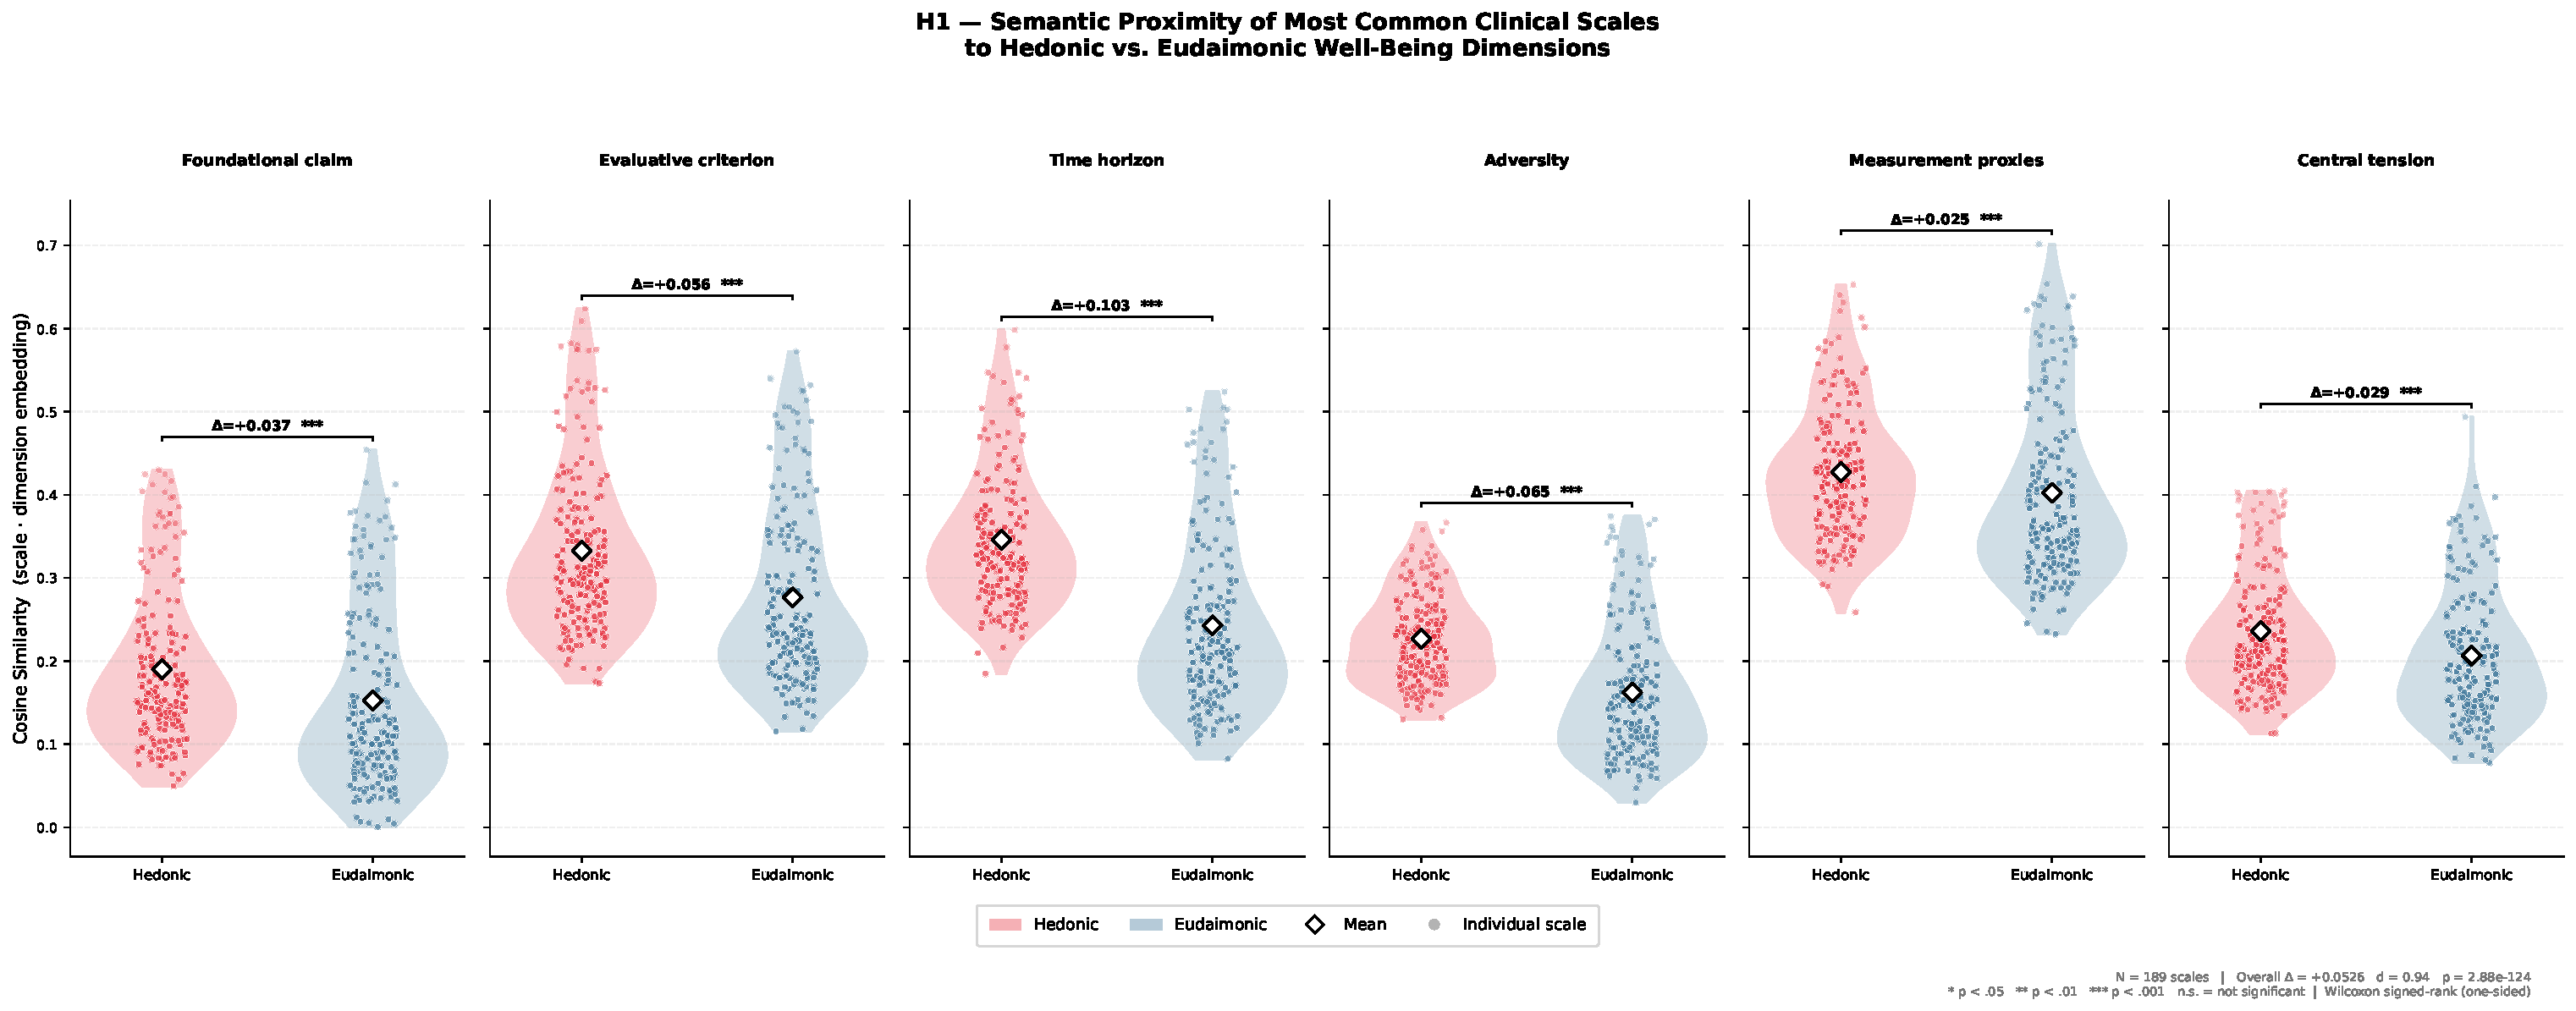
\includegraphics[width=\textwidth]{h1_violin_all.pdf}
    \caption{Distribution of cosine similarities between clinical scales and hedonic versus eudaimonic well-being poles across six dimensions}
    \label{fig:h1_violin_all}
    \floatnote{Diamonds represent arithmetic means. Red = hedonic pole; blue = eudaimonic pole. All differences are significant at $p < .001$ (Holm-corrected). Panels: (A) Foundational claim, (B) Evaluative criterion, (C) Time horizon, (D) Adversity, (E) Measurement proxies, (F) Central tension.}
\end{figure}

\begin{figure}[H]
    \centering
    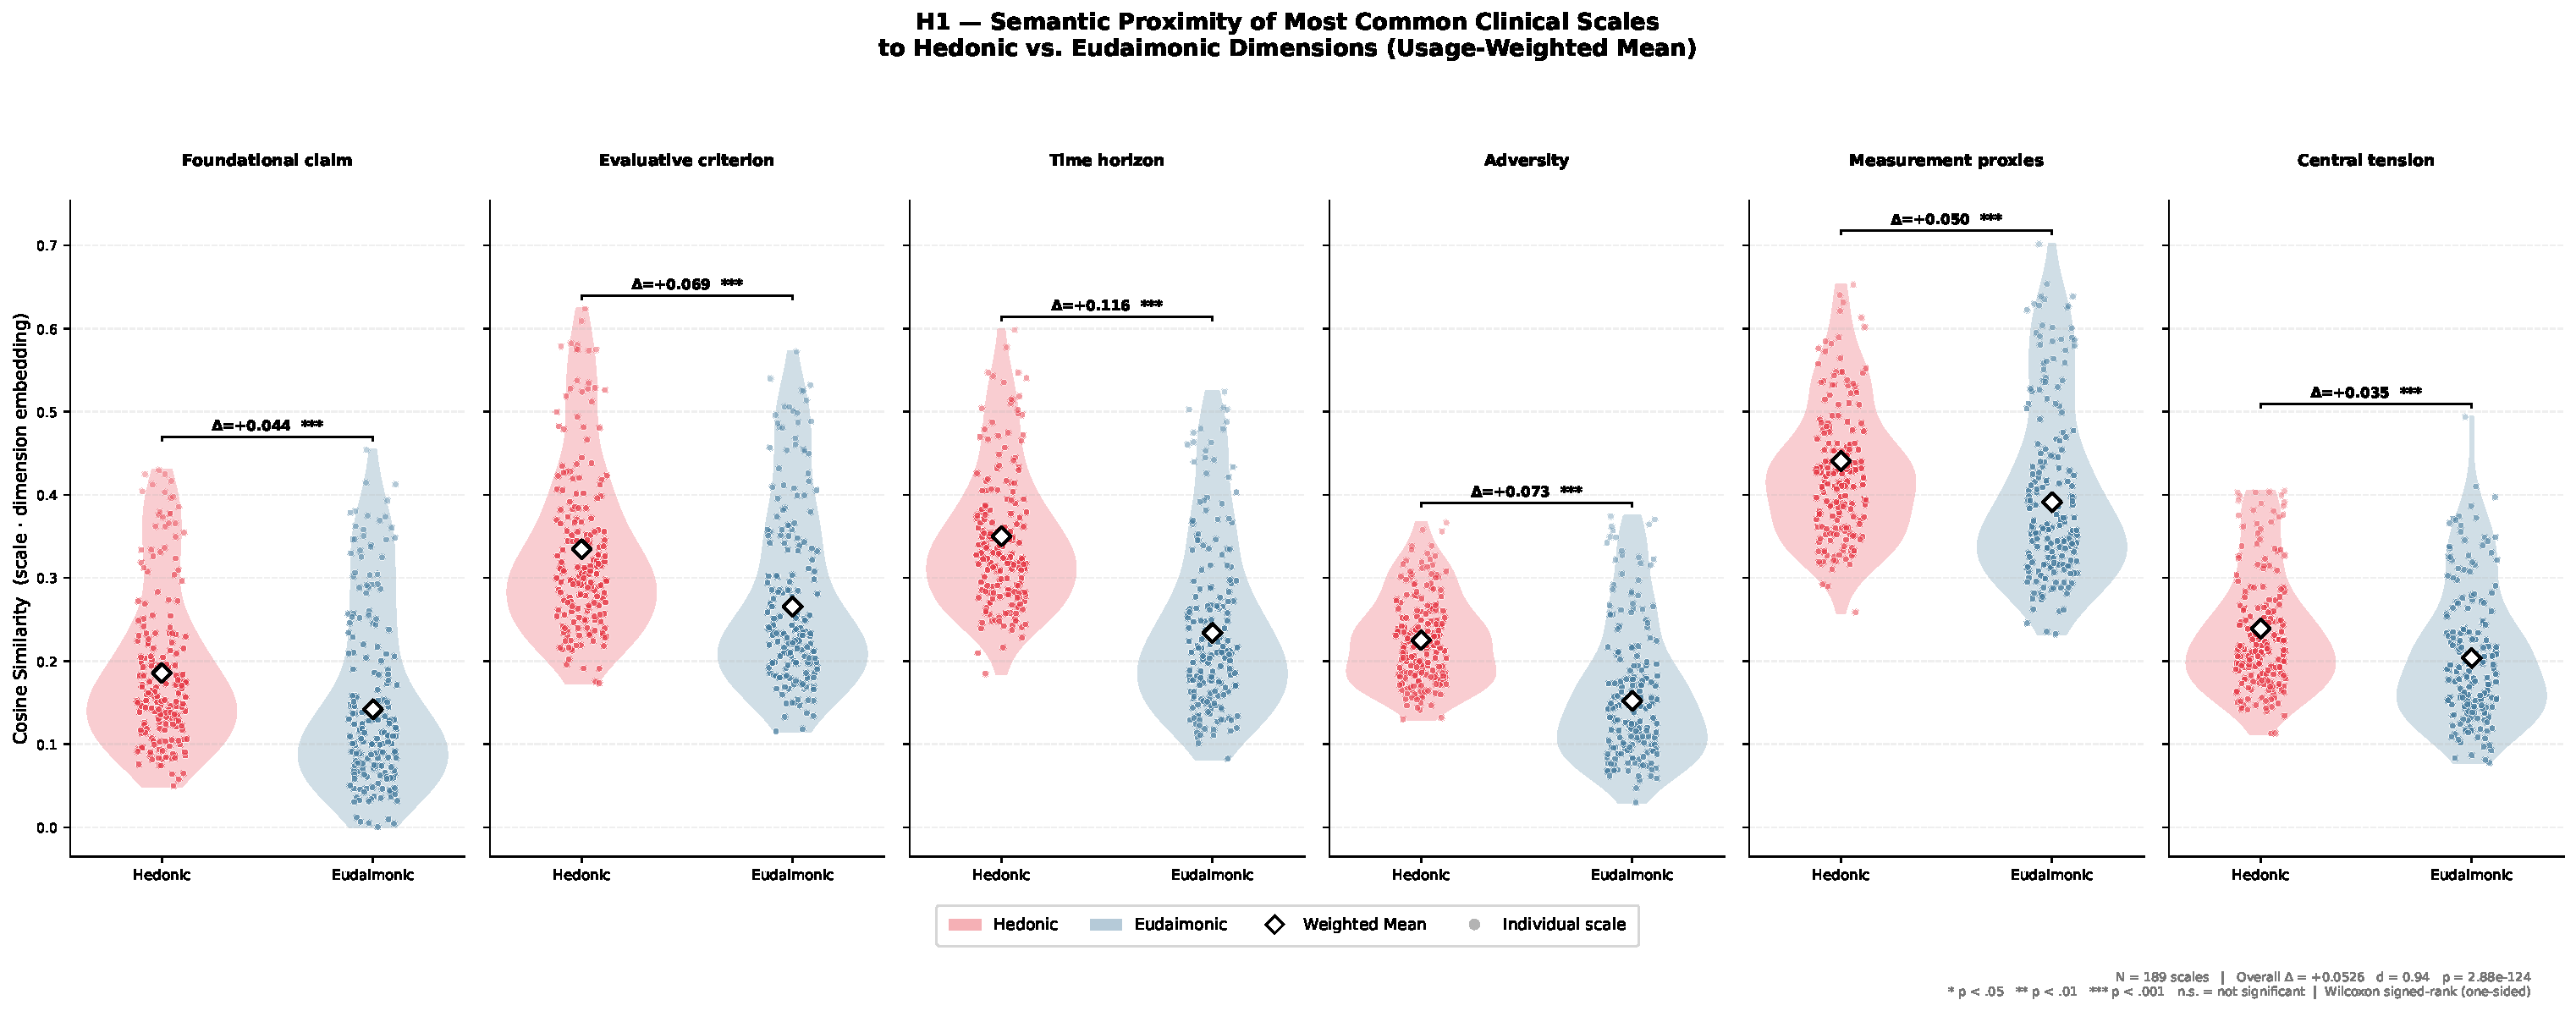
\includegraphics[width=\textwidth]{h1_violin_all_weighted.pdf}
    \caption{Usage-weighted cosine-similarity distributions for all clinical scales across six hedonic--eudaimonic dimensions}
    \label{fig:h1_violin_weighted}
    \floatnote{As Figure~\ref{fig:h1_violin_all}, but with diamonds representing usage-weighted means. Publication-frequency weighting slightly reduces the gap for less-cited eudaimonic instruments but preserves the overall pattern (weighted $\Delta = +0.056$, $d = 1.07$).}
\end{figure}

\begin{table}[H]
\centering
\caption{Per-dimension hedonic--eudaimonic comparison for all clinical scales}
\label{tab:h1_dims}
\small
\begin{tabular}{lcccccc}
\toprule
\textbf{Dimension} & \textbf{Mean $\Delta$} & \textbf{$d$} & \textbf{Wt.\ $\Delta$} & \textbf{Wt.\ $d$} & \textbf{$p_{\text{adj}}$} \\
\midrule
Foundational claim     & $+0.035$ & $1.03$ & $+0.030$ & $1.23$ & $< .001$ \\
Evaluative criterion   & $+0.055$ & $1.30$ & $+0.046$ & $1.27$ & $< .001$ \\
Time horizon           & $+0.103$ & $2.18$ & $+0.092$ & $1.98$ & $< .001$ \\
Adversity              & $+0.069$ & $1.29$ & $+0.068$ & $1.59$ & $< .001$ \\
Measurement proxies    & $+0.066$ & $0.86$ & $+0.075$ & $1.01$ & $< .001$ \\
Central tension        & $+0.030$ & $0.69$ & $+0.025$ & $0.64$ & $< .001$ \\
\midrule
\textbf{Overall}       & $\boldsymbol{+0.060}$ & $\boldsymbol{1.05}$ & $\boldsymbol{+0.056}$ & $\boldsymbol{1.07}$ & $\boldsymbol{< .001}$ \\
\bottomrule
\end{tabular}
\floatnote{Wt.\ = usage-weighted. All $p$-values Holm--Bonferroni corrected across six dimensions.}
\end{table}

The top-50 most-cited scales showed a marginally larger bias ($\Delta = +0.062$, $d = 1.13$), consistent with the hypothesis that the most widely adopted instruments are disproportionately hedonic.
Figure~\ref{fig:h1_top50} shows the violin plots for this subset.

\begin{figure}[H]
    \centering
    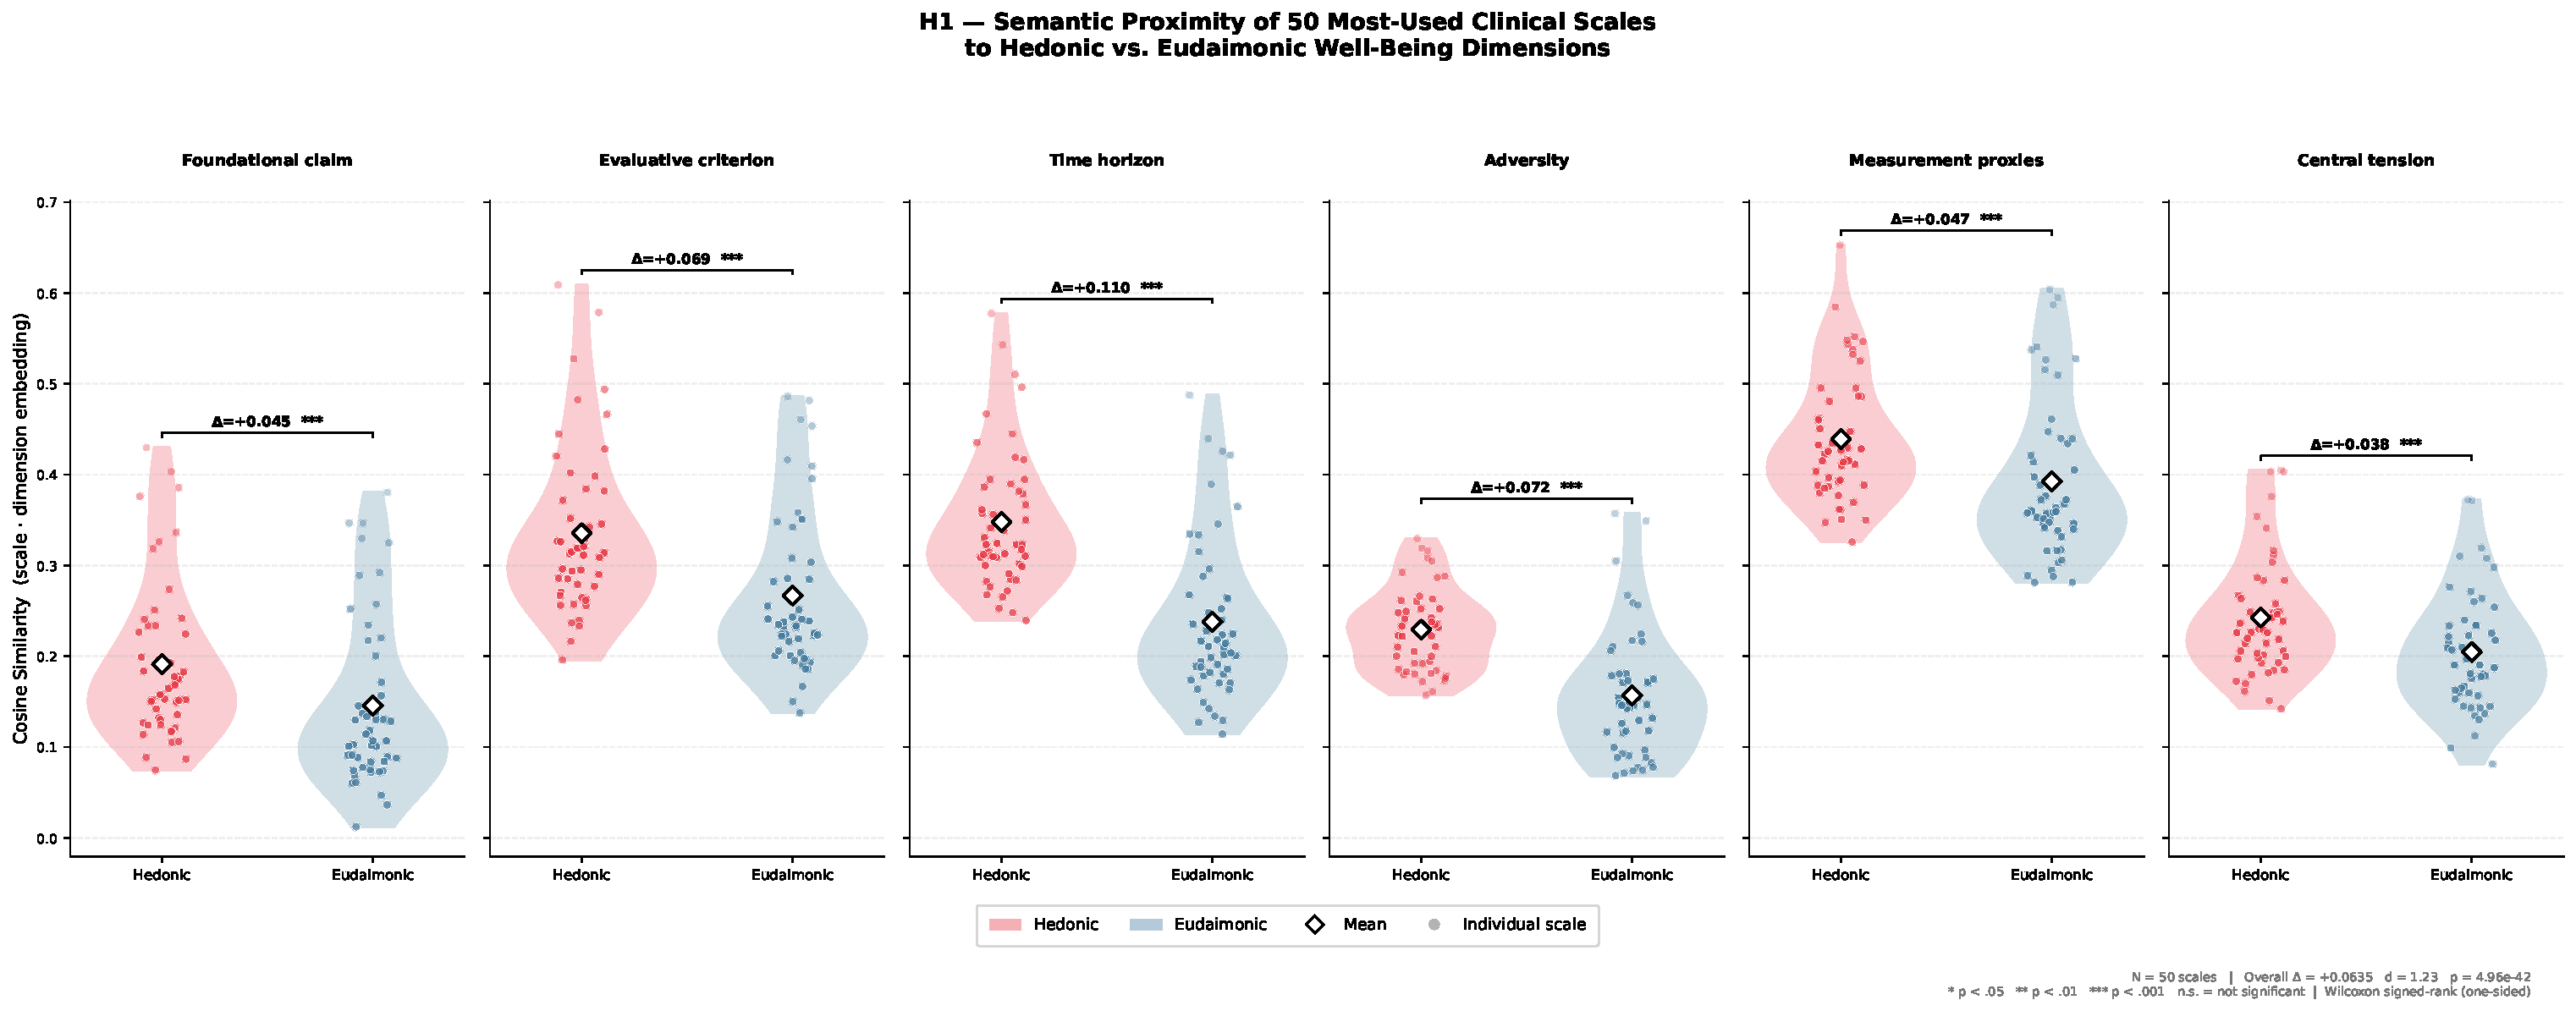
\includegraphics[width=\textwidth]{h1_violin_top50.pdf}
    \caption{Hedonic versus eudaimonic cosine similarities for the 50 most-cited clinical scales}
    \label{fig:h1_top50}
    \floatnote{The hedonic bias is slightly larger than in the full corpus ($d = 1.13$ vs.\ $1.05$), indicating that citation frequency amplifies the imbalance.}
\end{figure}

\subsection{H2: The Hedonic Bias Is Increasing Over Time}\label{sec:results-h2}

Temporal analysis of usage-weighted $\Delta$ from 2000 to 2025 revealed a significant positive trend for the aggregate series (slope $= +5.5 \times 10^{-4}$/year, $R^2 = .964$, $p < .001$; Figure~\ref{fig:h2_trends}).
All six individual dimensions also showed significant positive slopes (all $p < .001$ after Holm correction; Table~\ref{tab:h2_trends}).
The Mann-Kendall test confirmed the monotonic nature of the trend ($S = 321$, $p < .001$).

\begin{figure}[H]
    \centering
    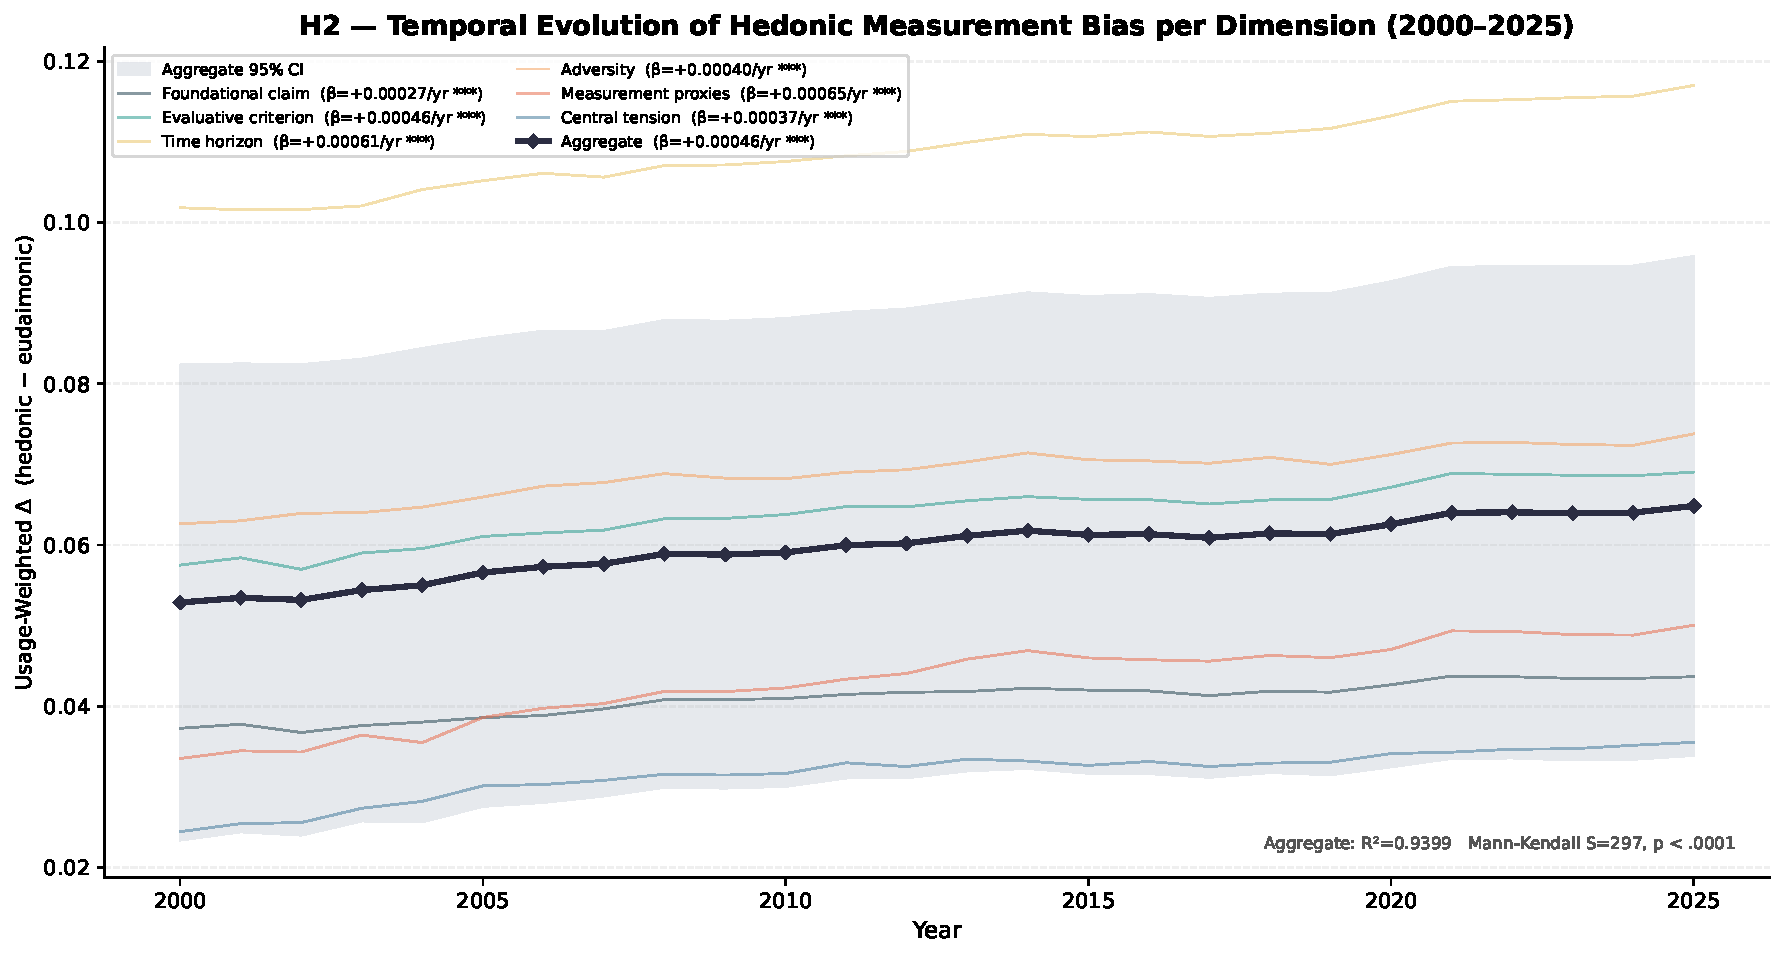
\includegraphics[width=\textwidth]{h2_dimension_trends.pdf}
    \caption{Temporal evolution of usage-weighted hedonic--eudaimonic differentials, 2000--2025}
    \label{fig:h2_trends}
    \floatnote{The shaded ribbon represents pointwise 95\% bootstrap CIs computed from cross-dimension variability. All trends are significantly positive ($p < .001$), indicating an increasing hedonic measurement bias.}
\end{figure}

\begin{figure}[H]
    \centering
    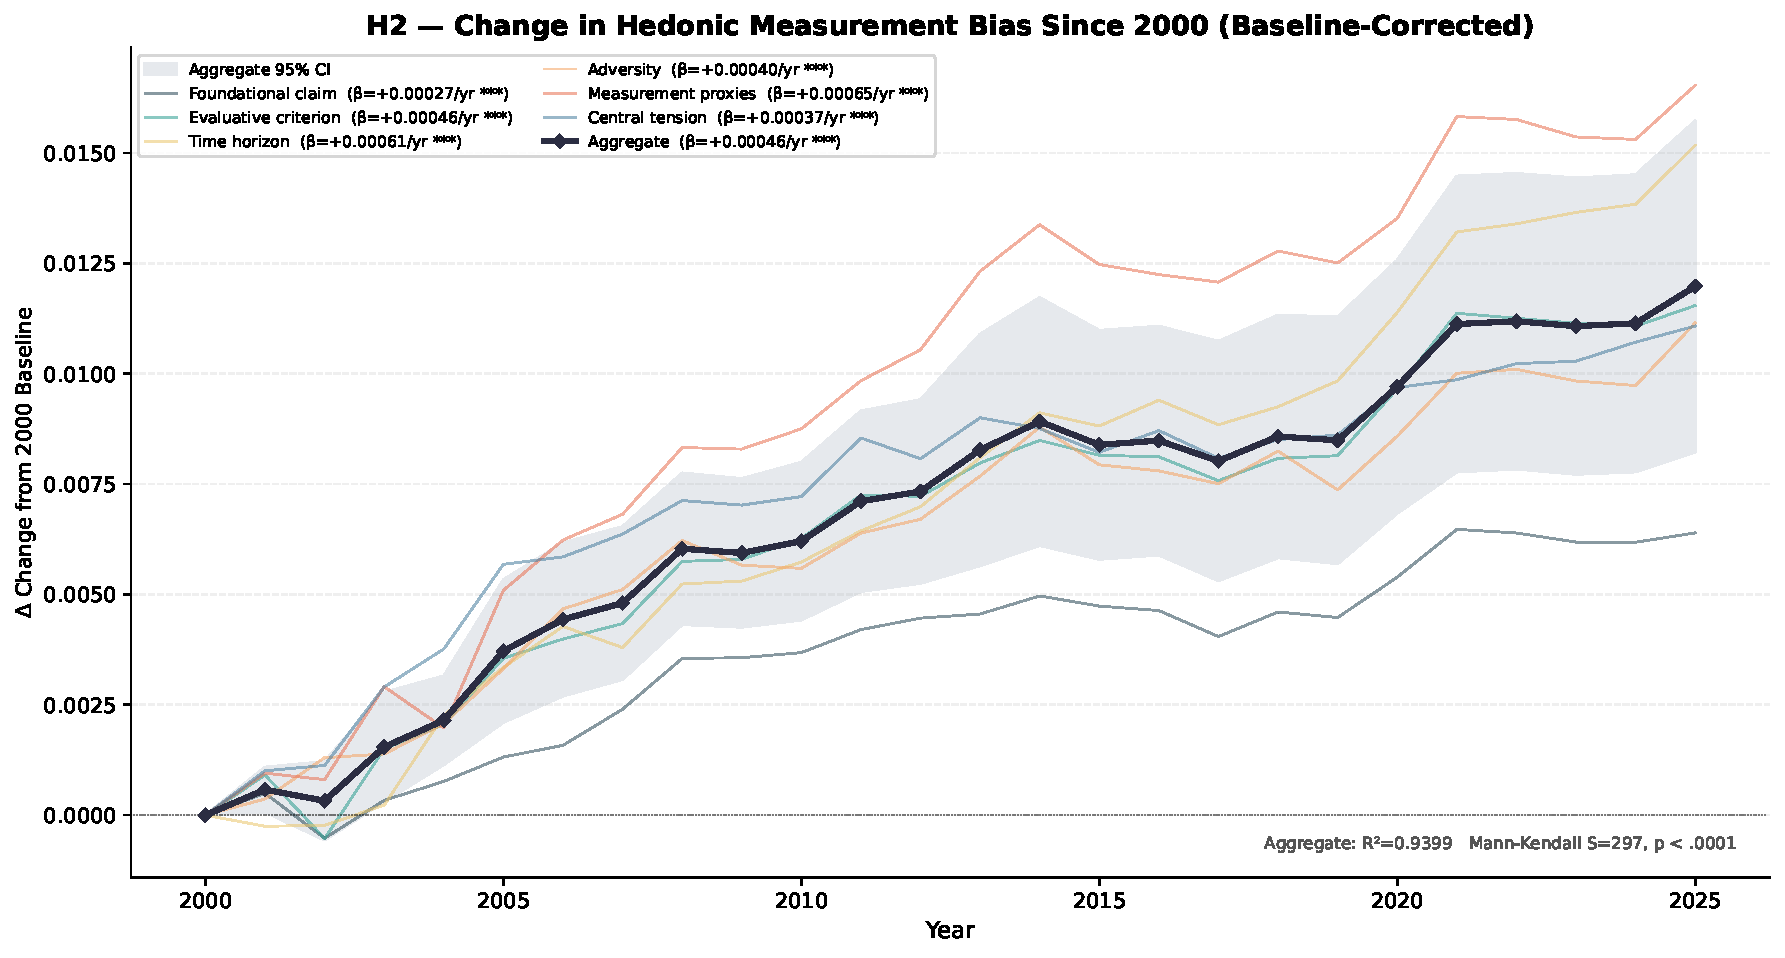
\includegraphics[width=\textwidth]{h2_baseline_corrected.pdf}
    \caption{Baseline-corrected temporal trends in hedonic--eudaimonic differentials}
    \label{fig:h2_baseline}
    \floatnote{Each series is adjusted by subtracting the year-2000 value. The aggregate hedonic bias increased by approximately $+0.014$ units over 25 years, with measurement proxies showing the largest absolute increase.}
\end{figure}

\begin{table}[H]
\centering
\caption{Per-dimension temporal trend statistics, 2000--2025}
\label{tab:h2_trends}
\small
\begin{tabular}{lcccccc}
\toprule
\textbf{Dimension} & \textbf{Slope ($\times 10^{-4}$/yr)} & \textbf{$R^2$} & \textbf{$p_{\text{OLS}}$} & \textbf{MK $S$} & \textbf{MK $p$} & \textbf{DW} \\
\midrule
Foundational claim   & $+1.49$ & $.955$ & $< .001$ & $313$ & $< .001$ & $0.46$ \\
Evaluative criterion & $+4.84$ & $.966$ & $< .001$ & $321$ & $< .001$ & $0.38$ \\
Time horizon         & $+4.67$ & $.981$ & $< .001$ & $323$ & $< .001$ & $0.47$ \\
Adversity            & $+5.34$ & $.964$ & $< .001$ & $319$ & $< .001$ & $0.33$ \\
Measurement proxies  & $+12.09$ & $.963$ & $< .001$ & $323$ & $< .001$ & $0.31$ \\
Central tension      & $+4.86$ & $.938$ & $< .001$ & $315$ & $< .001$ & $0.34$ \\
\midrule
\textbf{Aggregate}   & $\boldsymbol{+5.55}$ & $\boldsymbol{.964}$ & $\boldsymbol{< .001}$ & $\boldsymbol{321}$ & $\boldsymbol{< .001}$ & $\boldsymbol{0.33}$ \\
\bottomrule
\end{tabular}
\floatnote{OLS = ordinary least squares; MK = Mann-Kendall; DW = Durbin--Watson. All $p$-values Holm--Bonferroni corrected.}
\end{table}

The Durbin--Watson statistics (DW $= 0.31$--$0.47$) indicate substantial positive autocorrelation in the residuals, which is expected given the smooth, slowly evolving nature of publication patterns.
The converging evidence from both OLS and the non-parametric Mann-Kendall test---which makes no distributional assumptions---provides robust confirmation of the temporal trend.

\subsection{Post-Hoc and Robustness Analyses}\label{sec:results-posthoc}

\subsubsection{Permutation Test}

The observed mean $\Delta = +0.060$ fell in the right tail of the permutation null distribution (null mean $= +0.0003$, null SD $= 0.026$), yielding $p = .017$ (one-sided; Figure~\ref{fig:permutation}).
This confirms that the hedonic bias is not an artefact of the dimensional framework: randomly reassigning hedonic and eudaimonic labels produces near-zero average differences.

\begin{figure}[H]
    \centering
    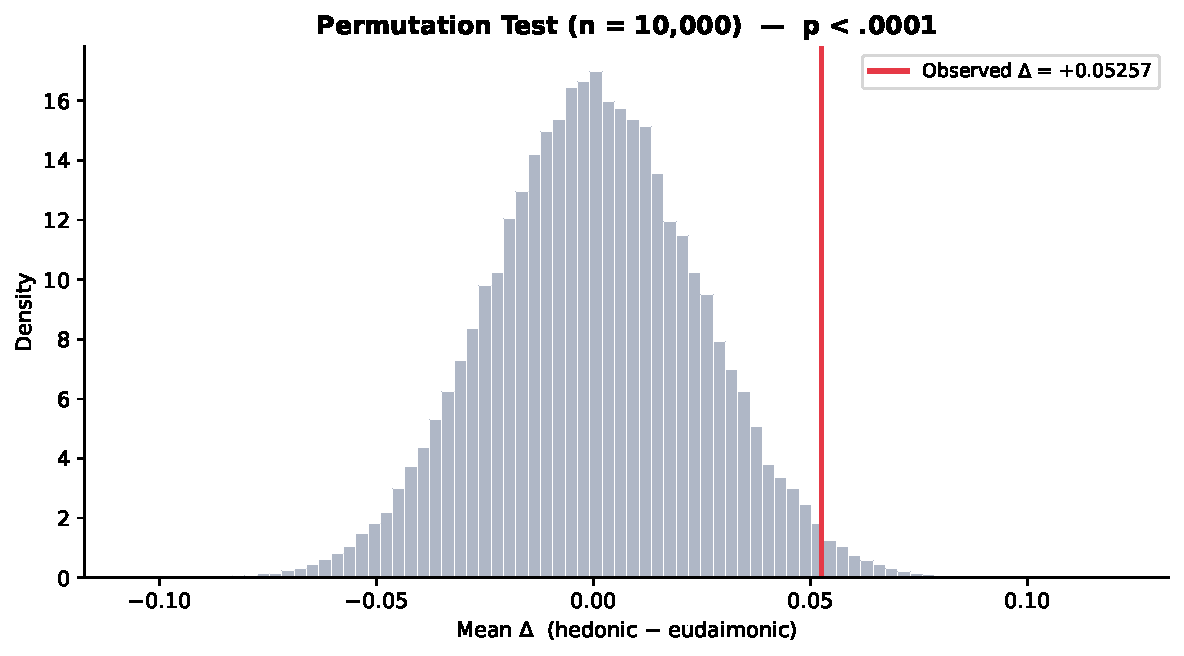
\includegraphics[width=0.75\textwidth]{posthoc_permutation.pdf}
    \caption{Permutation null distribution with observed hedonic--eudaimonic differential}
    \label{fig:permutation}
    \floatnote{$n = 10{,}000$ permutations; the red line indicates the observed $\Delta = +0.060$. The observed bias is significantly larger than expected under random labelling ($p = .017$).}
\end{figure}

\subsubsection{Sensitivity to Corpus Size}

The effect size was remarkably stable across corpus sizes: Cohen's $d_{\text{raw}}$ ranged from $1.31$ (top-20) to $1.53$ (top-150), with no evidence of dilution at larger $N$ (Table~\ref{tab:sensitivity}).
The usage-weighted mean $\Delta$ converged to approximately $+0.056$ for $N \geq 100$, indicating that the bias is a property of the scale ecosystem rather than a few outlier instruments.

\begin{table}[H]
\centering
\caption{Sensitivity analysis of effect size as a function of corpus size}
\label{tab:sensitivity}
\small
\begin{tabular}{rcccc}
\toprule
\textbf{Top-$N$} & \textbf{$\Delta_{\text{raw}}$} & \textbf{$d_{\text{raw}}$} & \textbf{$\Delta_{\text{weighted}}$} \\
\midrule
20  & $+0.058$ & $1.31$ & $+0.053$ \\
50  & $+0.062$ & $1.50$ & $+0.055$ \\
100 & $+0.065$ & $1.50$ & $+0.056$ \\
150 & $+0.063$ & $1.53$ & $+0.056$ \\
205 & $+0.060$ & $1.37$ & $+0.056$ \\
\bottomrule
\end{tabular}
\end{table}

\subsubsection{Domain-Level H1}

Seven of eight clinical domains showed a significant hedonic bias after Holm correction (Table~\ref{tab:domain_h1}).
The sole exception was Eudaimonic \& Flourishing ($\Delta = +0.011$, $d = 0.24$, $p_{\text{adj}} = .060$), which is expected given that this domain was specifically constructed to include scales targeting eudaimonic constructs.
Notably, even these scales showed a slight (non-significant) hedonic lean, suggesting that the semantic space of clinical measurement is pervasively tilted toward hedonic content.

The strongest hedonic loadings were observed for Substance Use \& Addiction ($d = 6.40$), Anxiety \& Stress ($d = 5.26$), and Mood \& Depression ($d = 4.59$).

\begin{table}[H]
\centering
\caption{Hedonic bias by clinical domain}
\label{tab:domain_h1}
\small
\begin{tabular}{lcccl}
\toprule
\textbf{Domain} & \textbf{$n$} & \textbf{$\Delta$} & \textbf{$d$} & \textbf{$p_{\text{adj}}$} \\
\midrule
Anxiety \& Stress                       & 19 & $+0.093$ & $5.26$ & $< .001$ \\
Mood \& Depression                      & 20 & $+0.094$ & $4.59$ & $< .001$ \\
Trauma \& PTSD                          & 10 & $+0.079$ & $4.34$ & $.003$ \\
General Distress \& Psychopathology     & 40 & $+0.079$ & $2.86$ & $< .001$ \\
Psychosis \& Severe Mental Illness      & 17 & $+0.077$ & $3.22$ & $< .001$ \\
Substance Use \& Addiction              &  8 & $+0.070$ & $6.40$ & $.008$ \\
Functional \& Quality of Life           & 50 & $+0.045$ & $1.29$ & $< .001$ \\
Eudaimonic \& Flourishing               & 41 & $+0.011$ & $0.24$ & $.060$ \\
\bottomrule
\end{tabular}
\floatnote{All $p$-values Holm--Bonferroni corrected across eight domains.}
\end{table}

\subsubsection{Domain-Level H2}

Domain-level temporal trends (Table~\\ref{tab:domain_h2}) revealed heterogeneous patterns.
Eudaimonic \& Flourishing showed the largest positive slope ($+0.007$/decade), reflecting the growing but still insufficient adoption of eudaimonic instruments.
General Distress \& Psychopathology ($+0.005$/decade) and Trauma \& PTSD ($+0.003$/decade) also showed significant positive trends.
Anxiety \& Stress and Psychosis showed small but significant negative slopes (total 25-year change $<\!-0.002$), possibly reflecting more nuanced instrumentation.

\begin{table}[H]
\centering
\caption{Temporal trends in hedonic bias by clinical domain}
\label{tab:domain_h2}
\small
\begin{tabular}{lccccl}
\toprule
\textbf{Domain} & \textbf{$n$} & \textbf{$\Delta$/decade} & \textbf{Total $\Delta$ (25\,yr)} & \textbf{$R^2$} & \textbf{$p_{\text{adj}}$} \\
\midrule
Eudaimonic \& Flourishing            & 41 & $+0.0070$ & $+0.018$ & $.980$ & $< .001$ \\
Gen.\ Distress \& Psychopathology    & 40 & $+0.0047$ & $+0.012$ & $.943$ & $< .001$ \\
Trauma \& PTSD                       & 10 & $+0.0028$ & $+0.007$ & $.977$ & $< .001$ \\
Mood \& Depression                   & 20 & $+0.0012$ & $+0.003$ & $.376$ & $.002$ \\
Substance Use \& Addiction           &  8 & $+0.0004$ & $+0.001$ & $.801$ & $< .001$ \\
Functional \& QoL                    & 50 & $-0.0004$ & $-0.001$ & $.052$ & $.261$ \\
Anxiety \& Stress                    & 19 & $-0.0010$ & $-0.002$ & $.938$ & $< .001$ \\
Psychosis \& SMI                     & 17 & $-0.0007$ & $-0.002$ & $.971$ & $< .001$ \\
\bottomrule
\end{tabular}
\floatnote{All $p$-values Holm--Bonferroni corrected. $\Delta$/decade = slope per decade; Total $\Delta$ = cumulative change over 25 years.}
\end{table}

\subsubsection{Usage--Bias Correlation}

The Spearman rank correlation between scale usage weight and mean $\Delta$ was $\rho = .134$ ($p = .056$), suggesting a marginally non-significant positive association.
While this does not reach conventional significance, the direction is consistent with the hypothesis that more widely adopted scales tend to carry greater hedonic loading (Figure~\ref{fig:scatter}).

\begin{figure}[H]
    \centering
    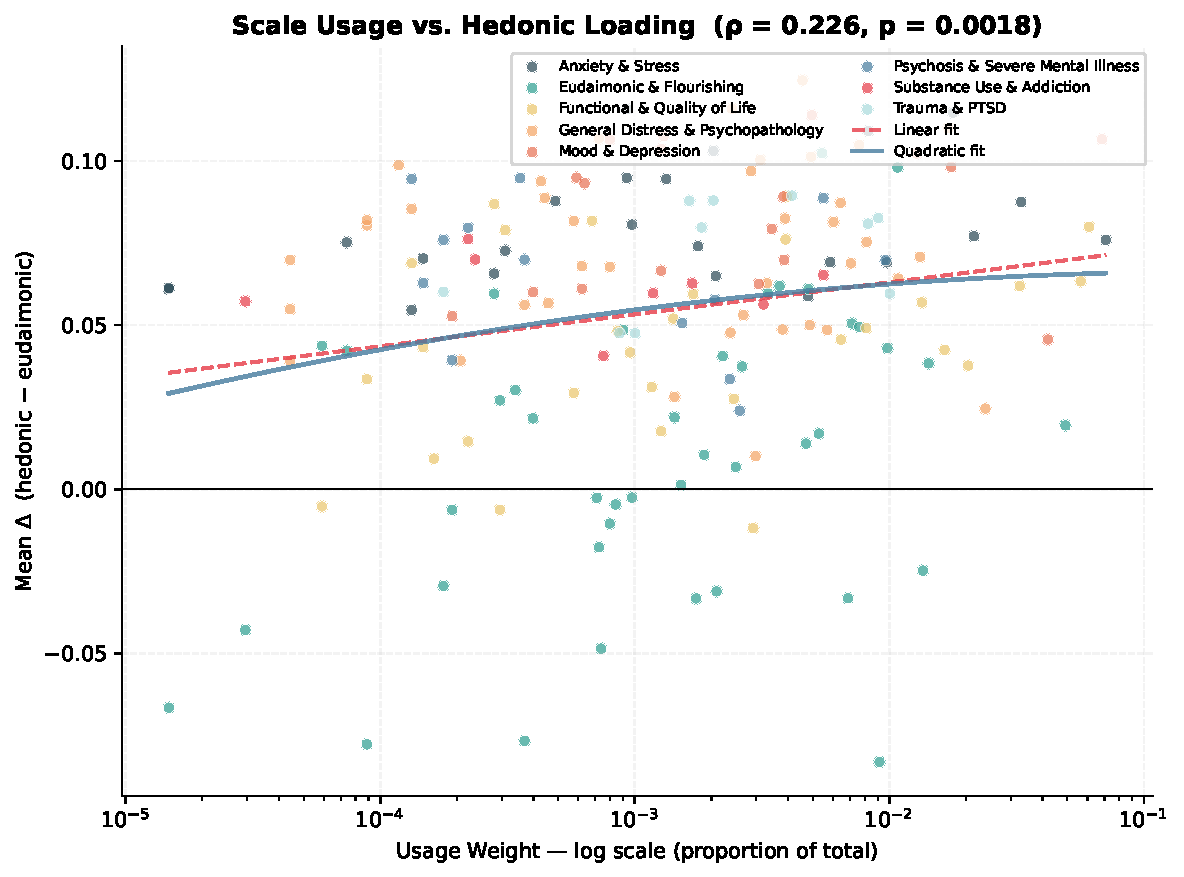
\includegraphics[width=0.75\textwidth]{posthoc_usage_scatter.pdf}
    \caption{Relationship between scale usage weight and hedonic loading}
    \label{fig:scatter}
    \floatnote{Each point represents one clinical scale, coloured by domain. Usage weights on log scale. Spearman $\rho = .134$, $p = .056$.}
\end{figure}

% ══════════════════════════════════════════════════════════════════════
\section{Discussion}\label{sec:discussion}
% ══════════════════════════════════════════════════════════════════════

\subsection{Summary of Findings}

This study provides the first large-scale, quantitative evidence that the Western mental healthcare assessment ecosystem is systematically biased toward hedonic conceptions of well-being and is converging further in that direction.
Using semantic embeddings of 205 clinical scales, we demonstrated that:
\begin{enumerate}
    \item Across all six theoretically derived hedonic--eudaimonic dimensions, clinical scales are significantly and substantially closer to hedonic poles ($d = 0.69$--$2.18$; all $p_{\text{adj}} < .001$).
    \item This bias is robust to usage-weighting, corpus size, and permutation-based null testing.
    \item The bias has \textit{increased} over the past 25 years, driven by the growing dominance of hedonically oriented instruments in the publication landscape.
    \item The bias is pervasive across clinical domains, with even nominally eudaimonic scales showing a slight (non-significant) hedonic lean.
\end{enumerate}

\subsection{Theoretical Implications}

Our findings converge with longstanding arguments in the well-being literature.
\citet{ryan2001happiness} and \citet{deci2000self} emphasised that hedonic and eudaimonic well-being are conceptually and empirically distinct, yet our data show that the measurement tools available to clinicians overwhelmingly probe only one side of this distinction.
\citet{keyes2002mental} called for a ``complete state model'' of mental health that includes both symptom absence and positive functioning; two decades later, our analysis suggests that clinical measurement has not caught up with this theoretical mandate.
Perhaps most strikingly, the WHO's own definition of mental health---emphasising self-realisation, productive functioning, and community contribution \citep{who2004mental}---is fundamentally eudaimonic, yet the instruments most widely deployed to assess mental health remain overwhelmingly hedonic.

The finding that the Time horizon dimension shows the largest effect ($d = 2.18$) is particularly striking.
Clinical scales predominantly assess present-moment states---current mood, recent symptom severity, functional status over the past two weeks---while eudaimonic conceptions emphasise long-term trajectories of growth, narrative identity, and purpose development
\citep{mcadams2001psychology, king2004benefit}.
This temporal myopia may cause clinicians and researchers to miss meaningful recovery that unfolds over months or years
\citep{tedeschi2004posttraumatic}.

\subsection{Practical Implications}

The increasing hedonic bias documented in H2 has direct consequences for clinical practice and health policy in Western mental healthcare:

\begin{enumerate}
    \item \textbf{Treatment evaluation:} If primary outcomes are hedonic (symptom reduction, mood improvement), interventions targeting meaning, autonomy, or growth may appear ineffective even when they produce substantial eudaimonic gains
    \citep{seligman2005positive, sin2009enhancing, wong2011what}.
    
    \item \textbf{Resource allocation:} Funding bodies and regulatory agencies that rely on standardised outcomes (e.g., NICE, FDA) may systematically undervalue eudaimonic interventions, creating a self-reinforcing cycle in which hedonic instruments receive more validation studies, further entrenching their dominance
    \citep{vittersø2016handbook}.
    
    \item \textbf{Patient perspectives:} Qualitative research consistently indicates that patients value meaning, purpose, and personal growth alongside---and sometimes above---symptom relief
    \citep{slade2010mental, davidson2008recovery}.
    Current measurement infrastructure cannot fully capture these priorities.
    
    \item \textbf{Assessment design:} Our findings provide an empirical foundation for developing next-generation assessment tools that balance hedonic and eudaimonic content.
    The dimensional framework (Table~\ref{tab:dimensions}) could guide item generation to ensure systematic coverage of both traditions.
\end{enumerate}

\subsection{Methodological Considerations}

The use of semantic embeddings as a measurement tool introduces both strengths and limitations.
On the strength side, embeddings provide a continuous, high-dimensional measure of semantic content that avoids binary categorisation.
The \texttt{text-embedding-3-large} model was trained on a diverse web corpus, capturing nuanced semantic relationships that keyword-based approaches would miss.

However, several methodological considerations warrant discussion.
First, embeddings reflect the distributional semantics of training data \citep{bender2021dangers}.
If the training corpus itself over-represents hedonic language in clinical contexts, the embeddings may amplify existing biases rather than providing a neutral measurement.
We mitigated this concern through the permutation test, which confirmed that the observed bias exceeds what would be expected under random labelling.

Second, the choice of six dimensions, while theoretically grounded, is necessarily selective.
Alternative dimensional frameworks might yield different effect sizes, though we expect the direction of the bias would be preserved given its consistency across all six dimensions tested.

Third, PubMed publication counts are an imperfect proxy for clinical usage.
Scales may be widely used in practice without generating proportional academic citations, and publication trends reflect research priorities rather than clinical deployment.

\subsection{Durbin--Watson and Autocorrelation}

The low Durbin--Watson statistics (DW $= 0.31$--$0.47$) indicate positive autocorrelation in the H2 residuals, which is expected for slowly evolving time series.
While this inflates the precision of OLS standard errors, three factors mitigate concern: (a) the Mann-Kendall test, which is non-parametric and robust to autocorrelation, independently confirms all trends; (b) bootstrap confidence intervals on slopes do not assume independence; and (c) the very high $R^2$ values ($> .93$) indicate that the linear trend captures the dominant signal, leaving little residual structure to exploit.

% ══════════════════════════════════════════════════════════════════════
\section{Limitations}\label{sec:limitations}
% ══════════════════════════════════════════════════════════════════════

\begin{enumerate}
    \item \textbf{Embedding model dependence:} Results may vary across embedding models, though the large, consistent effects observed here suggest robustness. Replication with alternative models (e.g., sentence-BERT, Cohere) would strengthen confidence.
    
    \item \textbf{Scale representation:} Scales were represented by brief textual descriptions rather than full item content. While this captures construct-level semantics, item-level analysis might reveal more nuanced patterns.
    
    \item \textbf{Dimensional framework:} The six dimensions were researcher-specified. Data-driven approaches (e.g., factor analysis of embedding similarity matrices) could complement this theory-driven framework.
    
    \item \textbf{PubMed bias:} Publication counts may not reflect clinical practice. Clinician surveys or electronic health record data would provide more direct evidence of scale adoption.
    
    \item \textbf{Language and culture:} All analyses were conducted in English. The hedonic--eudaimonic balance in clinical measurement may differ across languages and cultural contexts.
    
    \item \textbf{Causal interpretation:} The temporal trend (H2) is observational and cannot establish causation. The increasing hedonic bias may reflect changes in research priorities, funding structures, diagnostic classification systems, or population health needs.
\end{enumerate}

% ══════════════════════════════════════════════════════════════════════
\section{Conclusion}\label{sec:conclusion}
% ══════════════════════════════════════════════════════════════════════

This study provides robust, large-scale evidence that the Western mental healthcare assessment ecosystem systematically privileges hedonic over eudaimonic conceptions of well-being.
The bias is large (Cohen's $d > 1$), pervasive (present across all six dimensions and nearly all clinical domains), temporally increasing, and robust to multiple analytic strategies.
In short, the field's measurement infrastructure is converging toward hedonic optimisation.

These findings do not imply that hedonic measurement is unimportant---symptom relief and positive affect are genuine components of well-being.
Rather, they reveal a structural asymmetry between the WHO's eudaimonic definition of mental health and the hedonic instruments used to measure it.
Just as a thermometer calibrated only above $20\,^{\circ}$C would systematically underestimate cold, a measurement ecosystem that primarily captures hedonic states systematically underestimates the full spectrum of human flourishing.

Addressing this convergence will require concerted effort across multiple levels: developing and validating new eudaimonic instruments, incorporating eudaimonic outcomes into clinical trial protocols, and updating clinical guidelines to reflect the dual-continuum model of mental health.
The dimensional framework presented here offers a starting point for ensuring that future assessment tools provide balanced coverage of both hedonic and eudaimonic well-being.

% ══════════════════════════════════════════════════════════════════════
% References
% ══════════════════════════════════════════════════════════════════════
\newpage
\bibliographystyle{apalike}

\begin{thebibliography}{99}

\bibitem[Aristotle, 1999]{aristotle1999nicomachean}
Aristotle (1999).
\textit{Nicomachean Ethics} (T. Irwin, Trans., 2nd ed.).
Hackett Publishing.

\bibitem[Bender et~al., 2021]{bender2021dangers}
Bender, E.~M., Gebru, T., McMillan-Major, A., \& Shmitchell, S. (2021).
On the dangers of stochastic parrots: Can language models be too big?
\textit{Proceedings of FAccT '21}, 610--623.

\bibitem[Bhatia, 2019]{bhatia2019predicting}
Bhatia, S. (2019).
Predicting risk perception: New clues from data science.
\textit{Management Science, 65}(8), 3800--3823.

\bibitem[Bornmann \& Mutz, 2015]{bornmann2015growth}
Bornmann, L., \& Mutz, R. (2015).
Growth rates of modern science: A bibliometric analysis based on the number of publications and cited references.
\textit{Journal of the Association for Information Science and Technology, 66}(11), 2215--2222.

\bibitem[Brown et~al., 2020]{brown2020language}
Brown, T.~B., Mann, B., Ryder, N., et~al. (2020).
Language models are few-shot learners.
\textit{Advances in Neural Information Processing Systems, 33}, 1877--1901.

\bibitem[Caliskan et~al., 2017]{caliskan2017semantics}
Caliskan, A., Bryson, J.~J., \& Narayanan, A. (2017).
Semantics derived automatically from language corpora contain human-like biases.
\textit{Science, 356}(6334), 183--186.

\bibitem[Davidson et~al., 2008]{davidson2008recovery}
Davidson, L., Borg, M., Marin, I., Topor, A., Mezzina, R., \& Sells, D. (2008).
Processes of recovery in serious mental illness: Findings from a multinational study.
\textit{American Journal of Psychiatric Rehabilitation, 8}(3), 177--201.

\bibitem[Deci \& Ryan, 2000]{deci2000self}
Deci, E.~L., \& Ryan, R.~M. (2000).
The ``what'' and ``why'' of goal pursuits: Human needs and the self-determination of behavior.
\textit{Psychological Inquiry, 11}(4), 227--268.

\bibitem[Devlin et~al., 2019]{devlin2019bert}
Devlin, J., Chang, M.-W., Lee, K., \& Toutanova, K. (2019).
BERT: Pre-training of deep bidirectional transformers for language understanding.
\textit{Proceedings of NAACL-HLT}, 4171--4186.

\bibitem[Diener, 1984]{diener1984subjective}
Diener, E. (1984).
Subjective well-being.
\textit{Psychological Bulletin, 95}(3), 542--575.

\bibitem[Diener et~al., 1985]{diener1985satisfaction}
Diener, E., Emmons, R.~A., Larsen, R.~J., \& Griffin, S. (1985).
The Satisfaction With Life Scale.
\textit{Journal of Personality Assessment, 49}(1), 71--75.

\bibitem[Disabato et~al., 2016]{disabato2016different}
Disabato, D.~J., Goodman, F.~R., Kashdan, T.~B., Short, J.~L., \& Jarden, A. (2016).
Different types of well-being? A cross-cultural examination of hedonic and eudaimonic well-being.
\textit{Psychological Assessment, 28}(5), 471--482.

\bibitem[Grand et~al., 2022]{grand2022semantic}
Grand, G., Blank, I.~A., Pereira, F., \& Fedorenko, E. (2022).
Semantic projection recovers rich human knowledge of multiple object features from word embeddings.
\textit{Nature Human Behaviour, 6}(7), 975--987.

\bibitem[Holm, 1979]{holm1979simple}
Holm, S. (1979).
A simple sequentially rejective multiple test procedure.
\textit{Scandinavian Journal of Statistics, 6}(2), 65--70.

\bibitem[Huppert \& So, 2013]{huppert2009exploring}
Huppert, F.~A., \& So, T.~T.~C. (2013).
Flourishing across Europe: Application of a new conceptual framework for defining well-being.
\textit{Social Indicators Research, 110}(3), 837--861.

\bibitem[Huta \& Waterman, 2014]{huta2010pursuing}
Huta, V., \& Waterman, A.~S. (2014).
Eudaimonia and its distinction from hedonia: Developing a classification and terminology for understanding conceptual and operational definitions.
\textit{Journal of Happiness Studies, 15}(6), 1425--1456.

\bibitem[Kahneman et~al., 1999]{kahneman1999hedonic}
Kahneman, D., Diener, E., \& Schwarz, N. (Eds.) (1999).
\textit{Well-being: The Foundations of Hedonic Psychology}.
Russell Sage Foundation.

\bibitem[Kashdan et~al., 2008]{kashdan2008reconsidering}
Kashdan, T.~B., Biswas-Diener, R., \& King, L.~A. (2008).
Reconsidering happiness: The costs of distinguishing between hedonics and eudaimonia.
\textit{The Journal of Positive Psychology, 3}(4), 219--233.

\bibitem[Keyes, 2002]{keyes2002mental}
Keyes, C.~L.~M. (2002).
The mental health continuum: From languishing to flourishing in life.
\textit{Journal of Health and Social Behavior, 43}(2), 207--222.

\bibitem[King \& Hicks, 2021]{king2004benefit}
King, L.~A., \& Hicks, J.~A. (2021).
The science of meaning in life.
\textit{Annual Review of Psychology, 72}, 561--584.

\bibitem[Kjell et~al., 2023]{kjell2023text}
Kjell, O.~N.~E., Kjell, K., Garcia, D., \& Sikstr{\"o}m, S. (2023).
Predicting well-being using language models.
\textit{Psychological Methods, 28}(6), 1309--1326.

\bibitem[Larsen \& von Ins, 2010]{larsen2010rate}
Larsen, P.~O., \& von Ins, M. (2010).
The rate of growth in scientific publication and the decline in coverage provided by Science Citation Index.
\textit{Scientometrics, 84}(3), 575--603.

\bibitem[McAdams, 2001]{mcadams2001psychology}
McAdams, D.~P. (2001).
The psychology of life stories.
\textit{Review of General Psychology, 5}(2), 100--122.

\bibitem[Mikolov et~al., 2013]{mikolov2013distributed}
Mikolov, T., Sutskever, I., Chen, K., Corrado, G.~S., \& Dean, J. (2013).
Distributed representations of words and phrases and their compositionality.
\textit{Advances in Neural Information Processing Systems, 26}, 3111--3119.

\bibitem[Pennington et~al., 2014]{pennington2014glove}
Pennington, J., Socher, R., \& Manning, C.~D. (2014).
GloVe: Global vectors for word representation.
\textit{Proceedings of EMNLP}, 1532--1543.

\bibitem[Ryan \& Deci, 2001]{ryan2001happiness}
Ryan, R.~M., \& Deci, E.~L. (2001).
On happiness and human potentials: A review of research on hedonic and eudaimonic well-being.
\textit{Annual Review of Psychology, 52}(1), 141--166.

\bibitem[Ryff, 1989]{ryff1989happiness}
Ryff, C.~D. (1989).
Happiness is everything, or is it? Explorations on the meaning of psychological well-being.
\textit{Journal of Personality and Social Psychology, 57}(6), 1069--1081.

\bibitem[Seligman et~al., 2005]{seligman2005positive}
Seligman, M.~E.~P., Steen, T.~A., Park, N., \& Peterson, C. (2005).
Positive psychology progress: Empirical validation of interventions.
\textit{American Psychologist, 60}(5), 410--421.

\bibitem[Sin \& Lyubomirsky, 2009]{sin2009enhancing}
Sin, N.~L., \& Lyubomirsky, S. (2009).
Enhancing well-being and alleviating depressive symptoms with positive psychology interventions: A practice-friendly meta-analysis.
\textit{Journal of Clinical Psychology, 65}(5), 467--487.

\bibitem[Slade, 2010]{slade2010mental}
Slade, M. (2010).
Mental illness and well-being: The central importance of positive psychology and recovery approaches.
\textit{BMC Health Services Research, 10}(1), 26.

\bibitem[Steger et~al., 2006]{steger2006meaning}
Steger, M.~F., Frazier, P., Oishi, S., \& Kaler, M. (2006).
The Meaning in Life Questionnaire: Assessing the presence of and search for meaning in life.
\textit{Journal of Counseling Psychology, 53}(1), 80--93.

\bibitem[Tedeschi \& Calhoun, 2004]{tedeschi2004posttraumatic}
Tedeschi, R.~G., \& Calhoun, L.~G. (2004).
Posttraumatic growth: Conceptual foundations and empirical evidence.
\textit{Psychological Inquiry, 15}(1), 1--18.

\bibitem[Vittersø, 2016]{vittersø2016handbook}
Vittersø, J. (Ed.) (2016).
\textit{Handbook of Eudaimonic Well-Being}.
Springer.

\bibitem[Waterman, 1993]{waterman1993eudaimonia}
Waterman, A.~S. (1993).
Two conceptions of happiness: Contrasts of personal expressiveness (eudaimonia) and hedonic enjoyment.
\textit{Journal of Personality and Social Psychology, 64}(4), 678--691.

\bibitem[Watson et~al., 1988]{watson1988panas}
Watson, D., Clark, L.~A., \& Tellegen, A. (1988).
Development and validation of brief measures of positive and negative affect: The PANAS scales.
\textit{Journal of Personality and Social Psychology, 54}(6), 1063--1070.

\bibitem[Wong, 2011]{wong2011what}
Wong, P.~T.~P. (2011).
What is existential positive psychology?
\textit{International Journal of Existential Psychology and Psychotherapy, 4}(1), 1--10.

\bibitem[World Health Organization, 2004]{who2004mental}
World Health Organization (2004).
\textit{Promoting Mental Health: Concepts, Emerging Evidence, Practice (Summary Report)}.
Geneva: World Health Organization.

\end{thebibliography}

% ══════════════════════════════════════════════════════════════════════
\newpage
\appendix
\section*{Supplementary Materials}
\addcontentsline{toc}{section}{Supplementary Materials}
% ══════════════════════════════════════════════════════════════════════

\subsection*{S1.\ Usage-Weighted Violin Plot (Top-50 Scales)}

\begin{figure}[H]
    \centering
    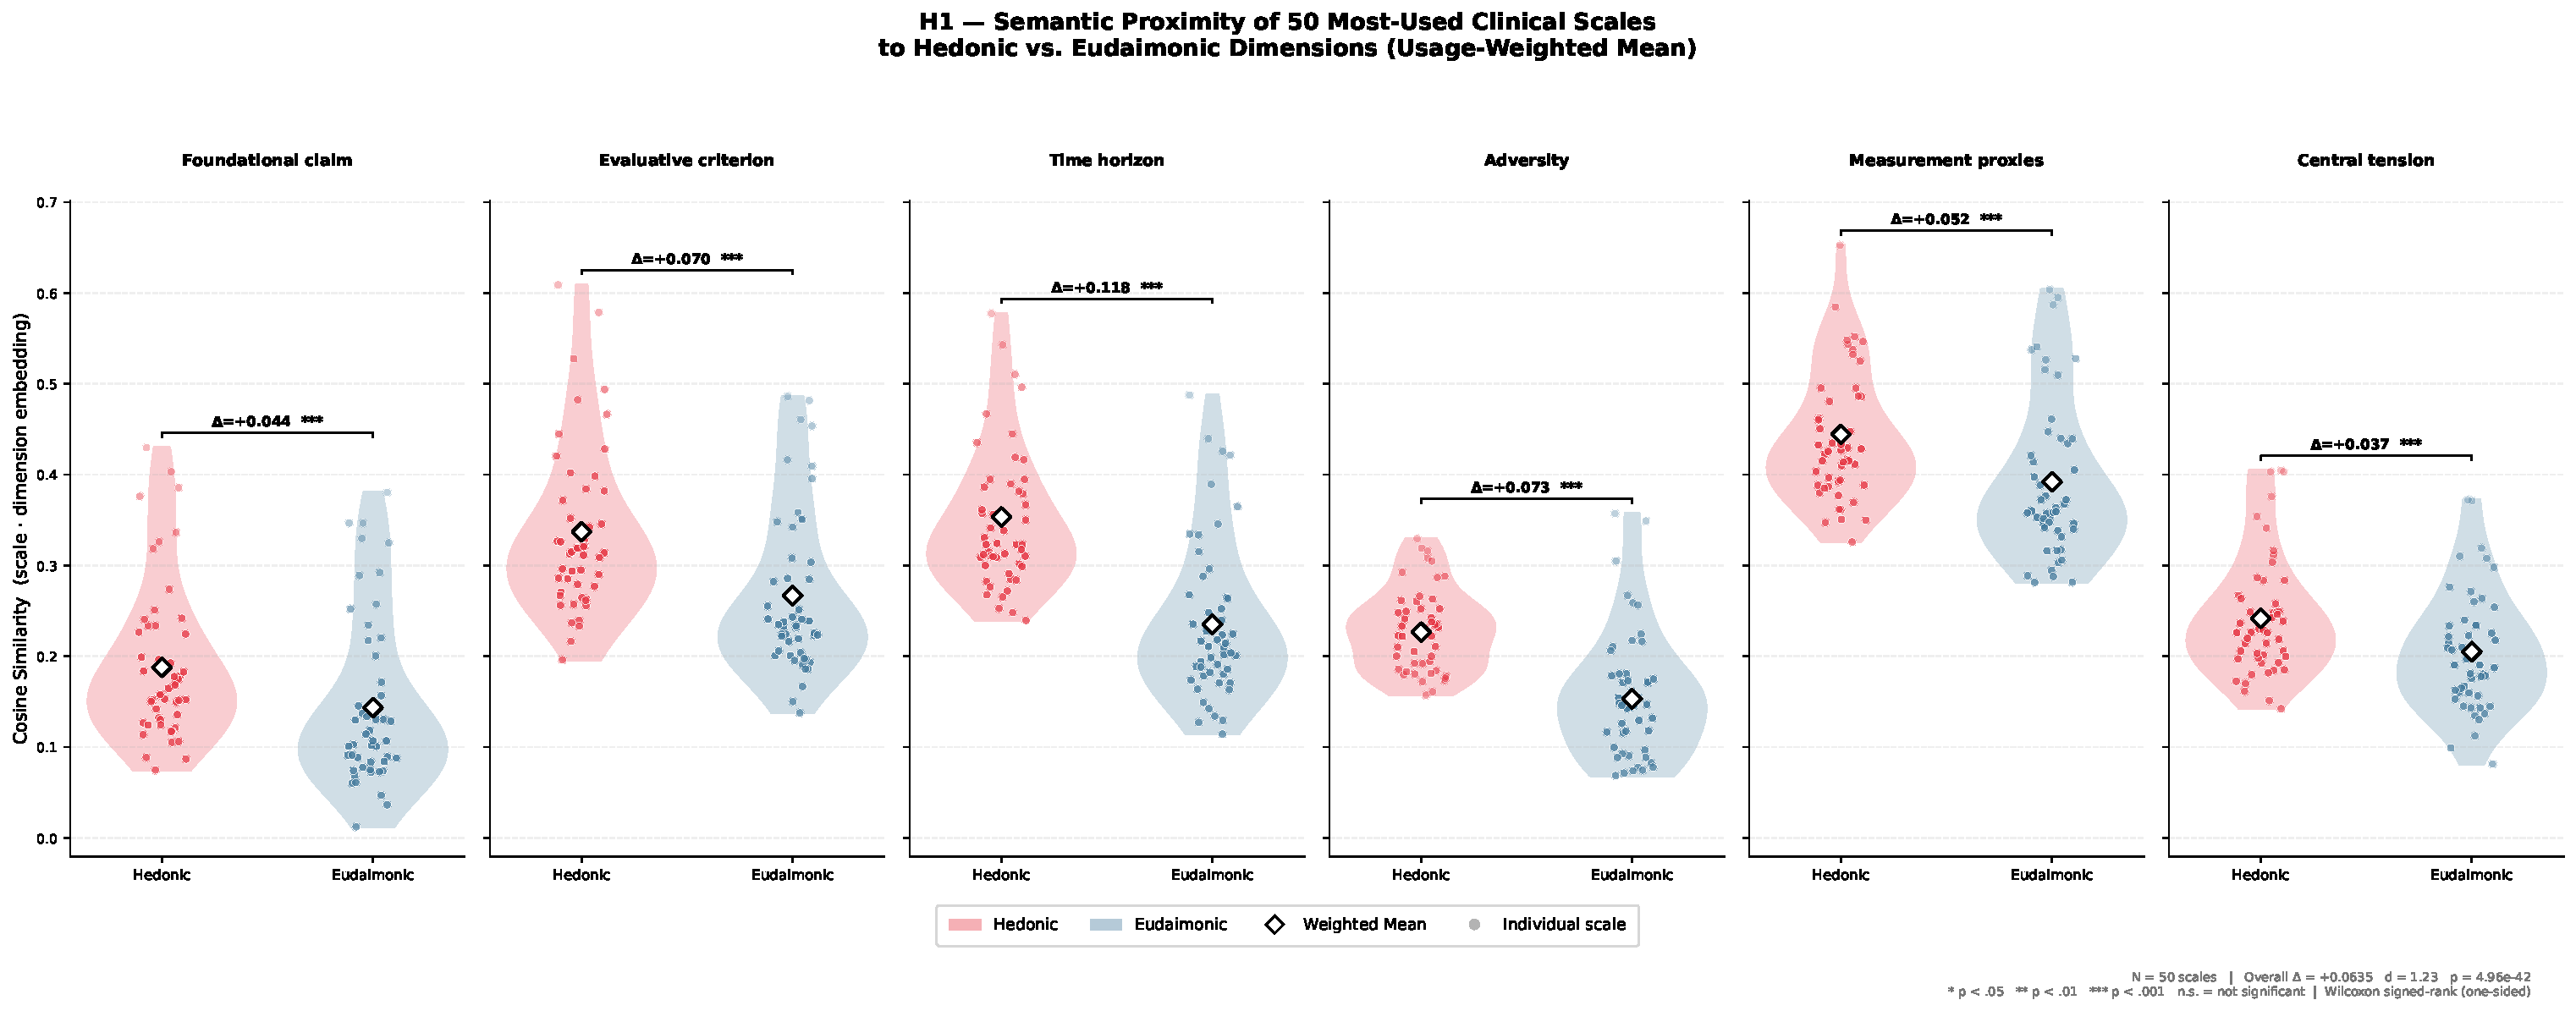
\includegraphics[width=\textwidth]{h1_violin_top50_weighted.pdf}
    \caption{Usage-weighted violin plot for the 50 most-cited clinical scales}
    \label{fig:s1_top50_weighted}
    \floatnote{As Figure~\ref{fig:h1_top50}, but with diamonds indicating usage-weighted means rather than arithmetic means (weighted $\Delta = +0.055$, $d = 1.06$).}
\end{figure}

\subsection*{S2.\ Four-Panel Comparison of All Sub-Analyses}

\begin{figure}[H]
    \centering
    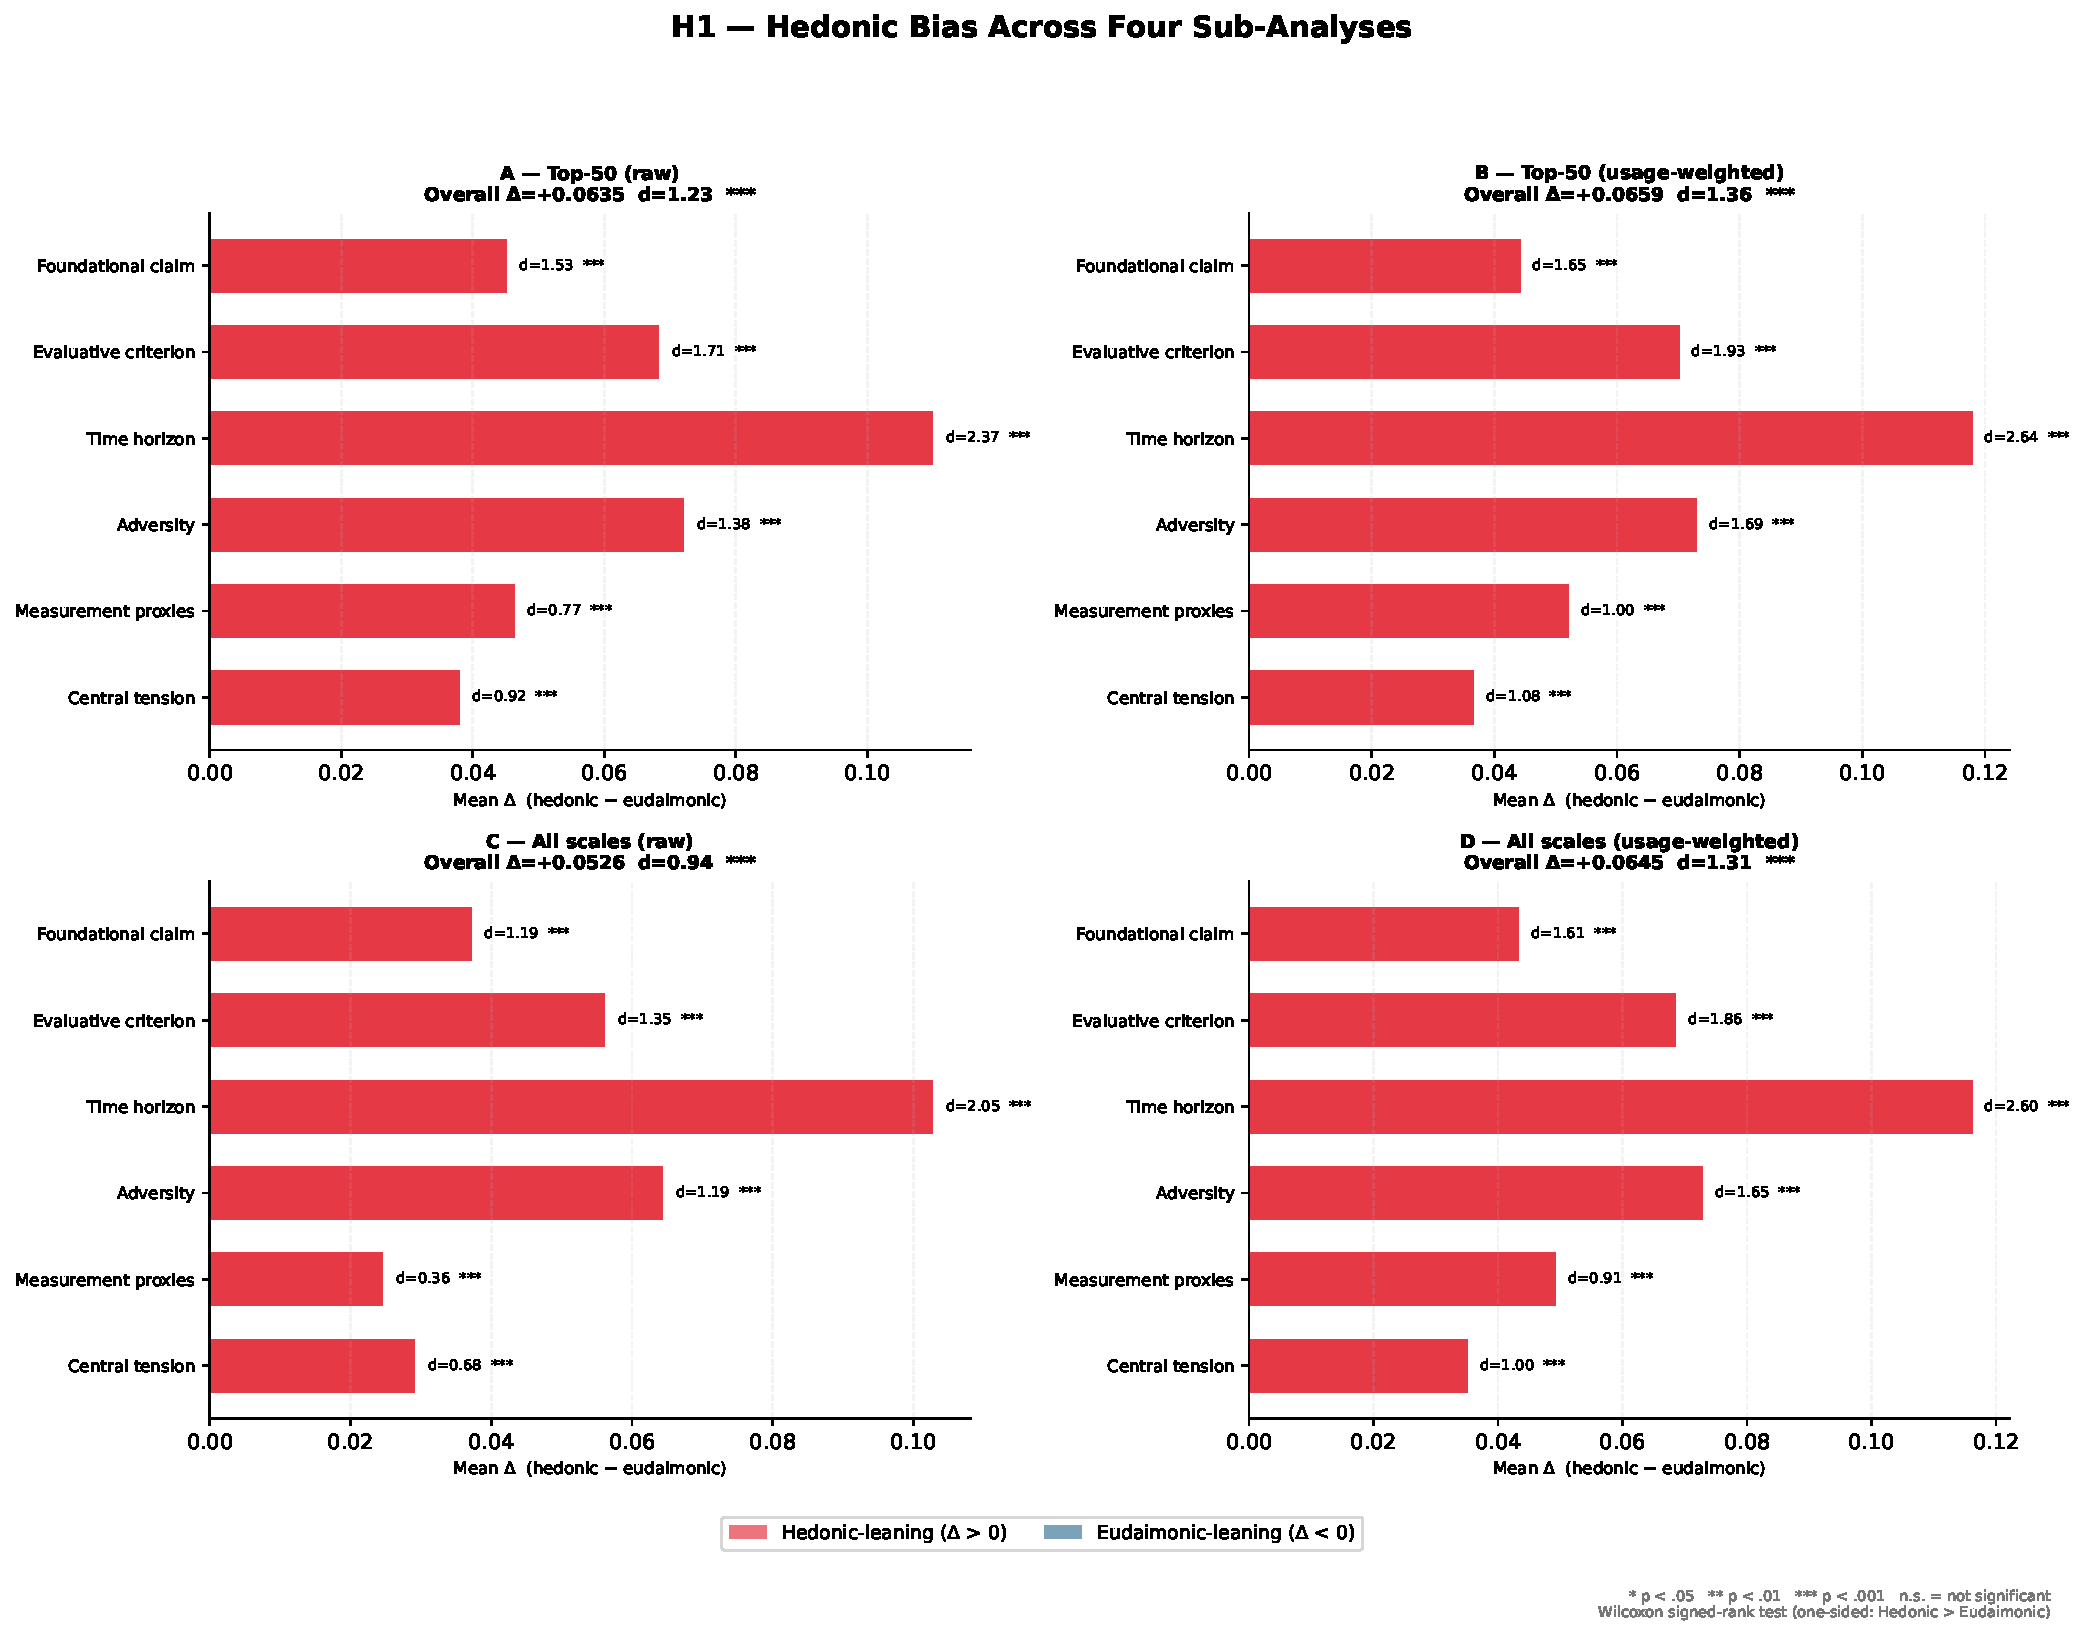
\includegraphics[width=\textwidth]{h1_four_panel.pdf}
    \caption{Four-panel comparison of all H1 sub-analyses}
    \label{fig:s2_four_panel}
    \floatnote{Per-dimension mean $\Delta$ and Cohen's $d$ for all four H1 sub-analyses: (A) Top-50 raw, (B) Top-50 usage-weighted, (C) All scales raw, (D) All scales usage-weighted.}
\end{figure}

\subsection*{S3.\ Effect-Size Comparison}

\begin{figure}[H]
    \centering
    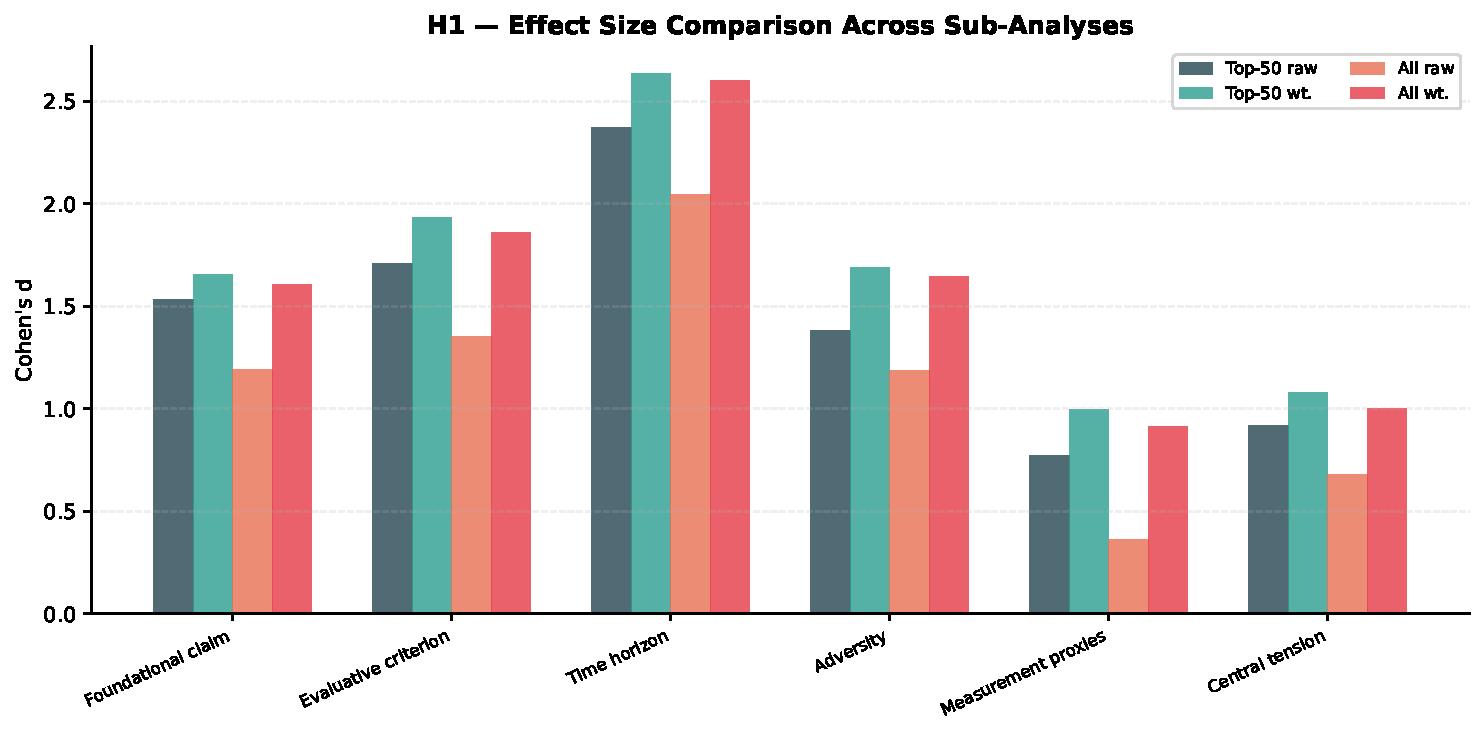
\includegraphics[width=\textwidth]{h1_effect_sizes.pdf}
    \caption{Cohen's $d$ by dimension across all four sub-analyses}
    \label{fig:s3_effect_sizes}
    \floatnote{The consistent pattern across raw and weighted analyses, and across top-50 and full corpus, indicates the hedonic bias is not driven by a few outlier scales.}
\end{figure}

\subsection*{S4.\ Domain-Level H1 Bar Chart}

\begin{figure}[H]
    \centering
    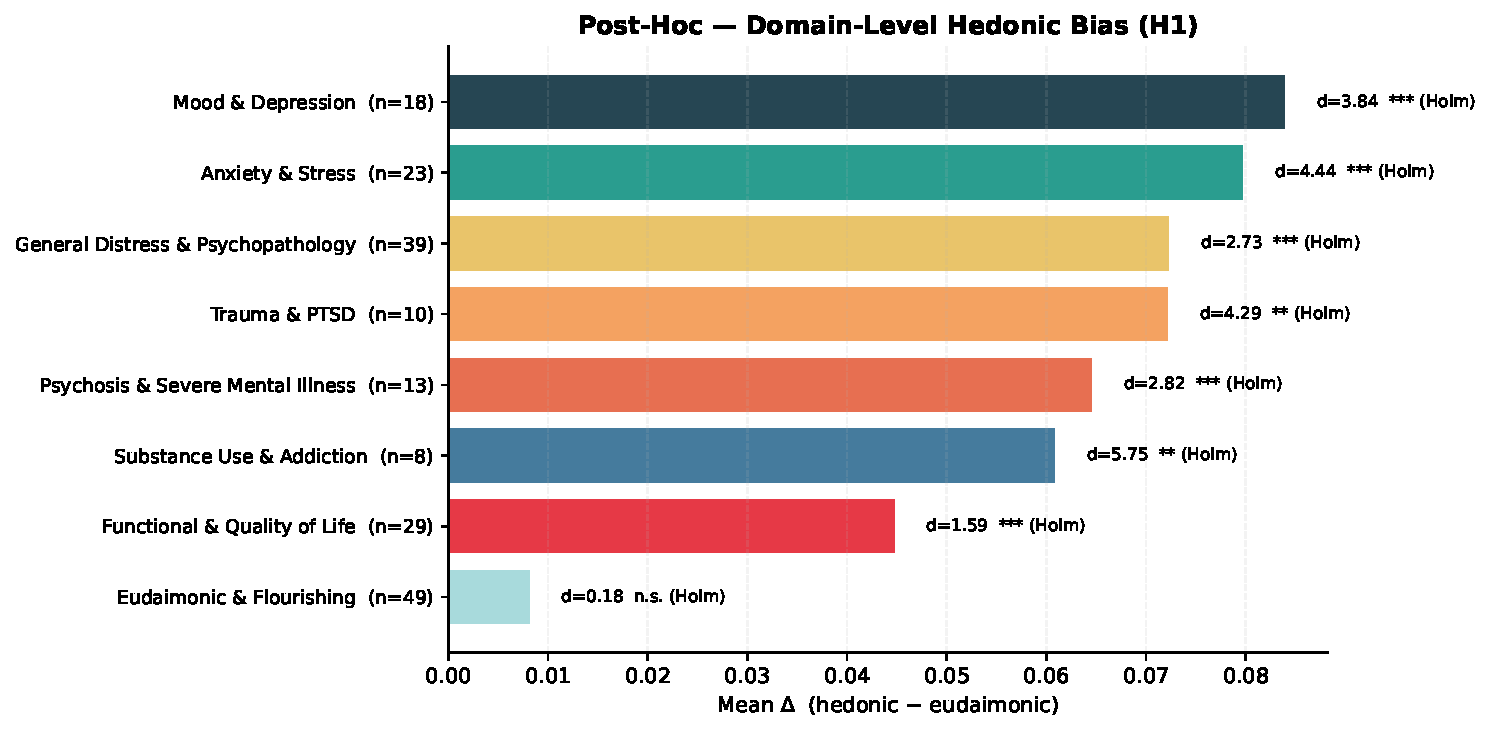
\includegraphics[width=0.85\textwidth]{posthoc_domain_h1.pdf}
    \caption{Domain-level hedonic bias sorted by effect size}
    \label{fig:s4_domain_h1}
    \floatnote{Mean $\Delta$ and Cohen's $d$ by clinical domain. All domains except Eudaimonic \& Flourishing show significant hedonic bias after Holm correction.}
\end{figure}

\subsection*{S5.\ Domain-Level H2 Small Multiples}

\begin{figure}[H]
    \centering
    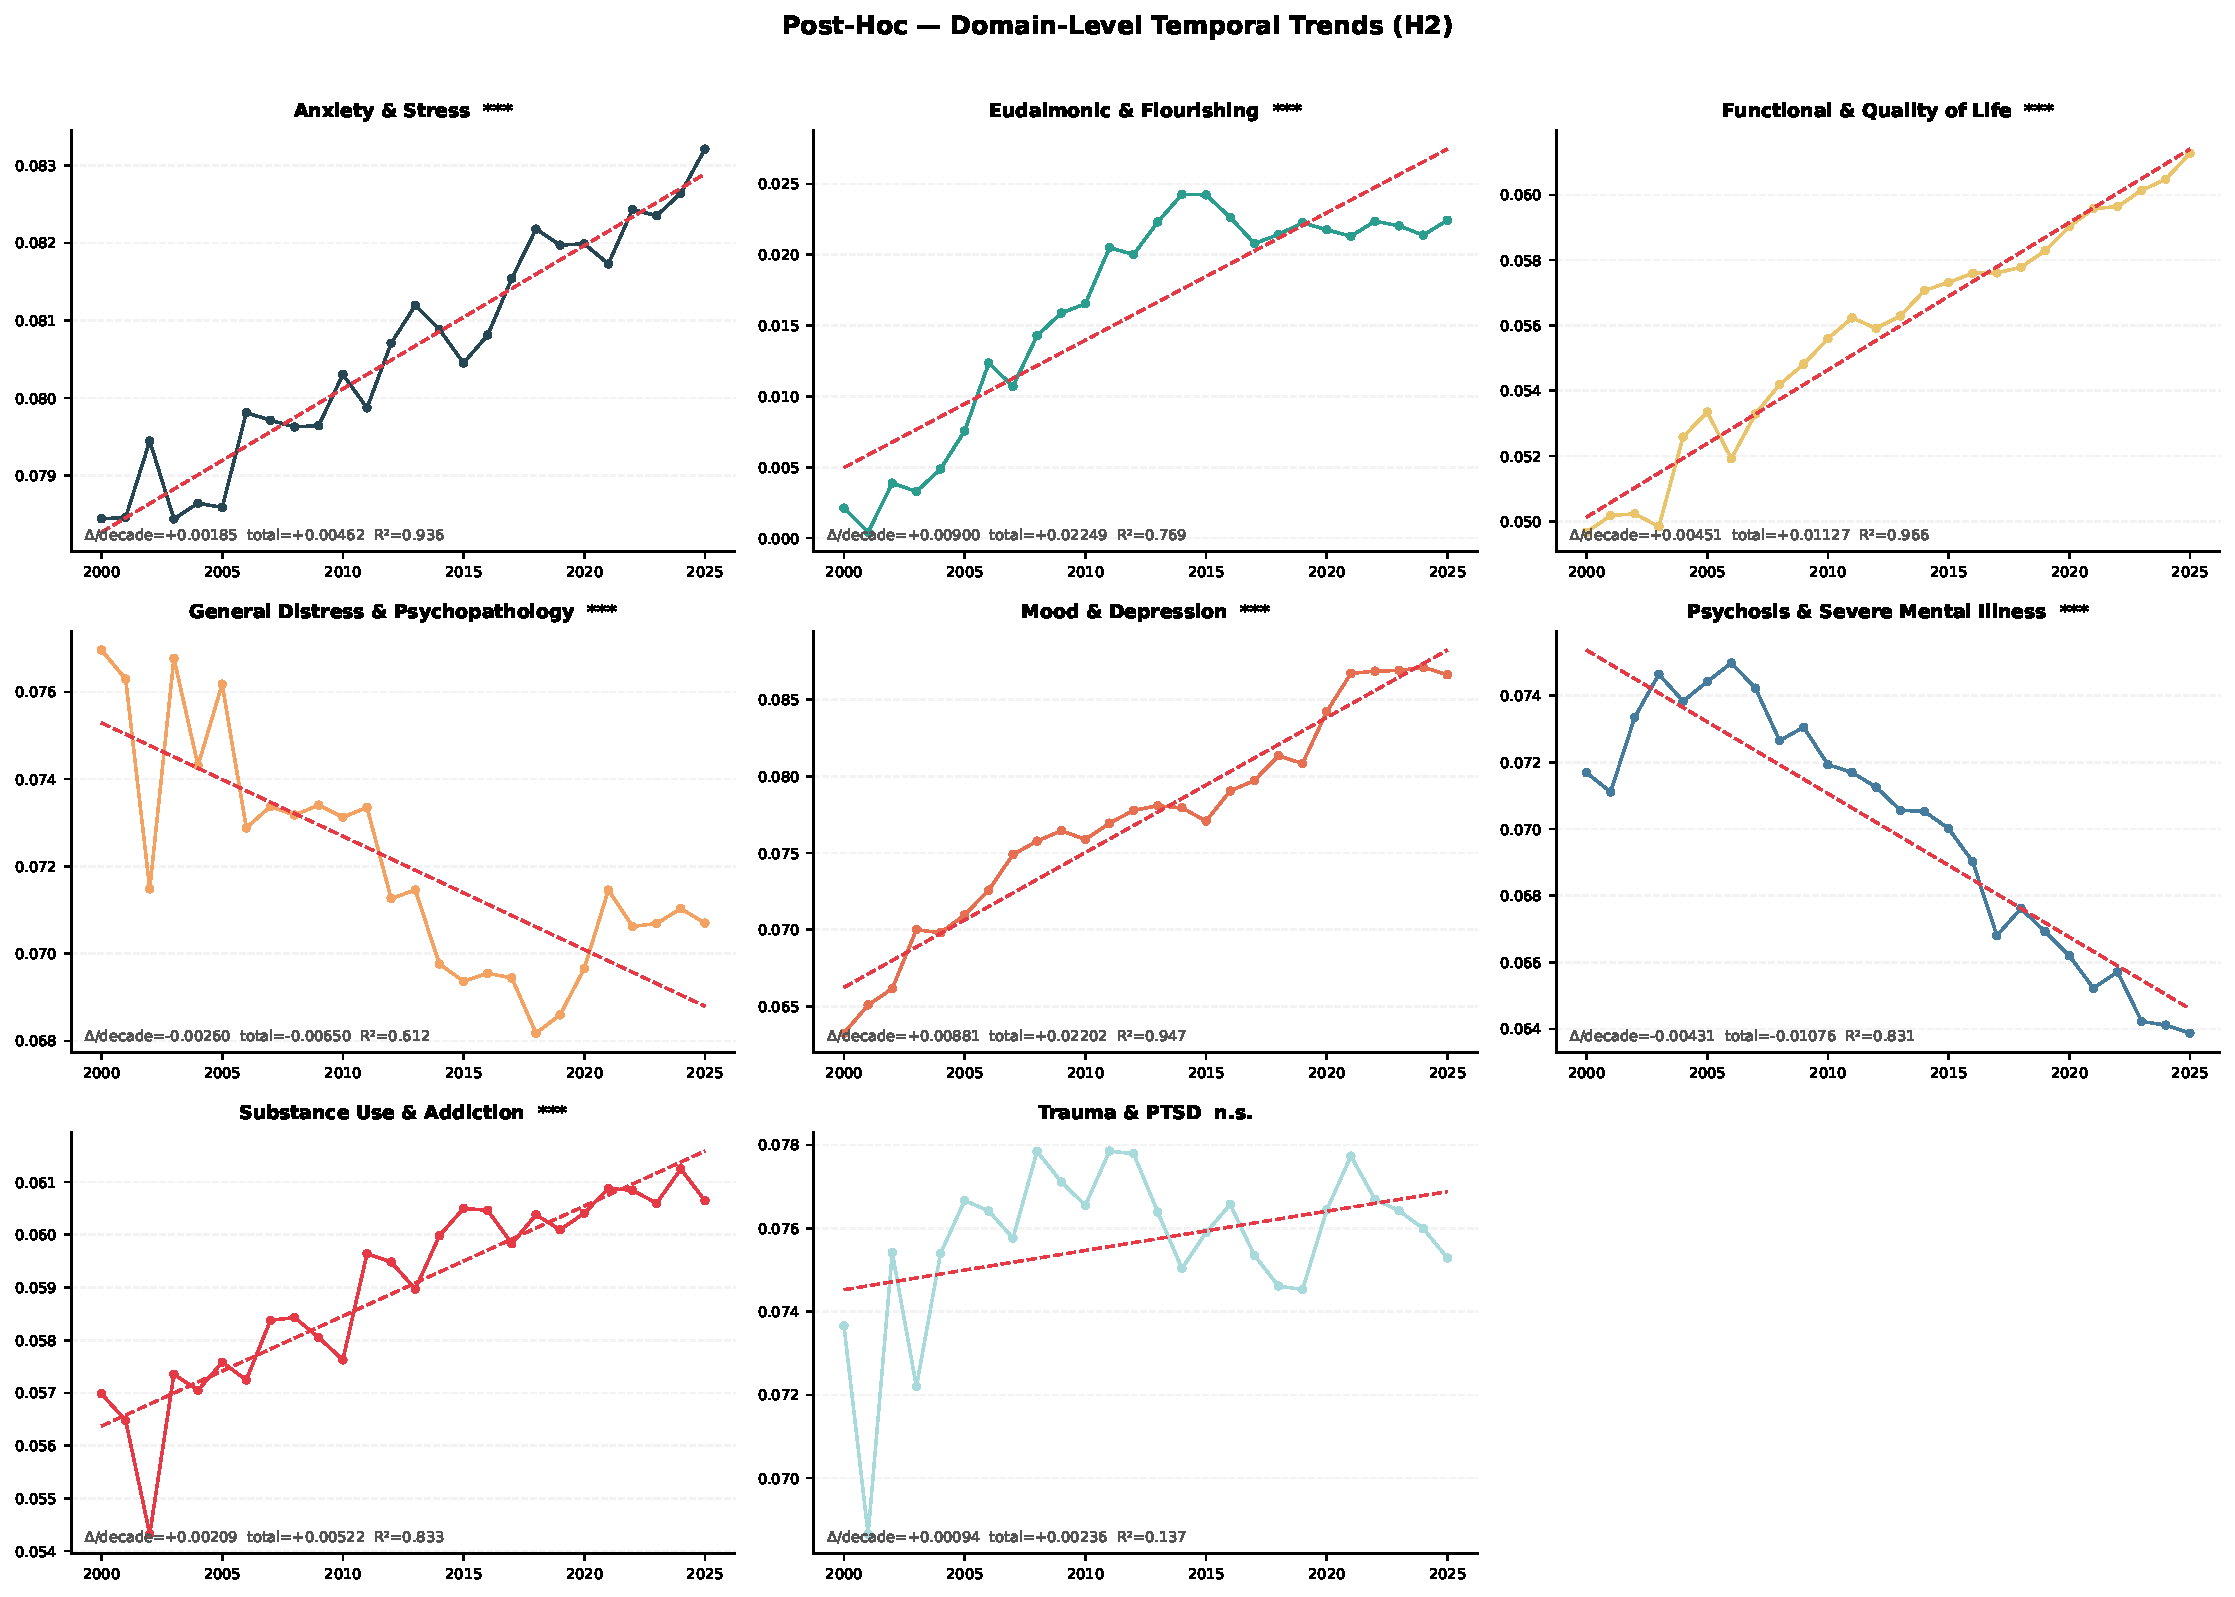
\includegraphics[width=\textwidth]{posthoc_domain_h2.pdf}
    \caption{Per-domain temporal trends in usage-weighted hedonic--eudaimonic differentials, 2000--2025}
    \label{fig:s5_domain_h2}
    \floatnote{Dashed red lines show OLS fits. Most domains show increasing hedonic bias; Anxiety and Psychosis show flat or slightly decreasing trends.}
\end{figure}

\subsection*{S6.\ Sensitivity to Corpus Size}

\begin{figure}[H]
    \centering
    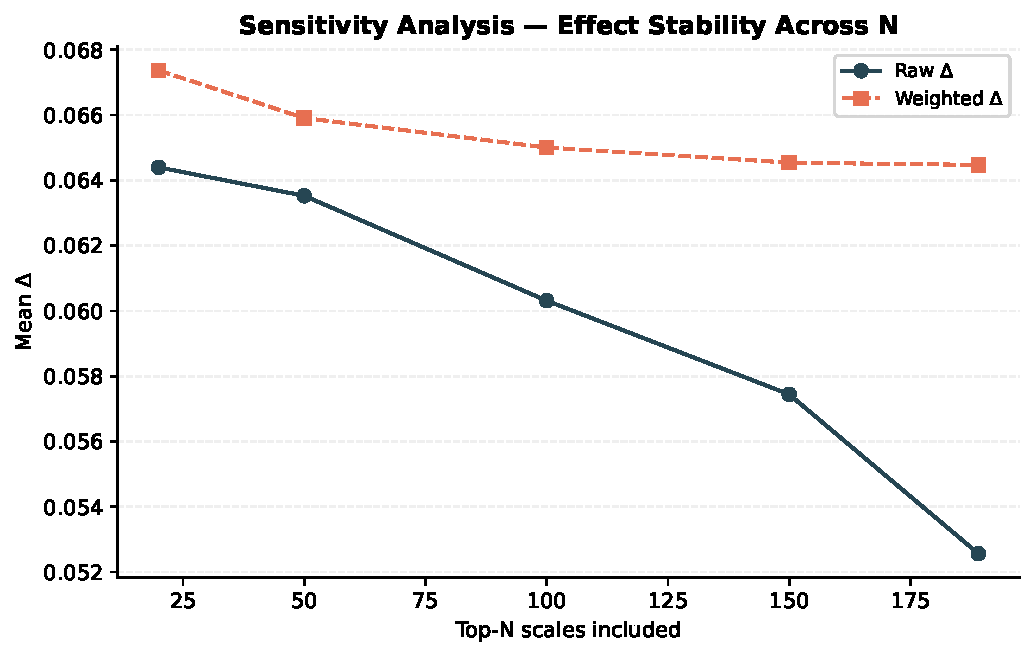
\includegraphics[width=0.7\textwidth]{posthoc_sensitivity_n.pdf}
    \caption{Sensitivity of hedonic bias estimates to corpus size}
    \label{fig:s6_sensitivity}
    \floatnote{Mean $\Delta$ (raw and usage-weighted) as a function of the number of scales included (top-$N$ by citation count). The effect is stable across $N = 20$--$205$, confirming that the hedonic bias is a systemic property of the clinical scale ecosystem.}
\end{figure}

\end{document}
